% ******************************* PhD Thesis Template **************************
% Please have a look at the README.md file for info on how to use the template

\documentclass[a4paper,12pt,times,authoryear,print]{PhDThesisPSnPDF}

% ******************************************************************************
% ******************************* Class Options ********************************
% *********************** See README for more details **************************
% ******************************************************************************

% `a4paper'(The University of Cambridge PhD thesis guidelines recommends a page
% size a4 - default option) or `a5paper': A5 Paper size is also allowed as per
% the Cambridge University Engineering Deparment guidelines for PhD thesis
%
% `11pt' or `12pt'(default): Font Size 10pt is NOT recommended by the University
% guidelines
%
% `oneside' or `twoside'(default): Printing double side (twoside) or single
% side.
%
% `print': Use `print' for print version with appropriate margins and page
% layout. Leaving the options field blank will activate Online version.
%
% `index': For index at the end of the thesis
%
% `draftclassic': For draft mode without loading any images (same as draft in book)
%
% `draft': Special draft mode with line numbers, images, and water mark with
% timestamp and custom text. Position of the text can also be modified.
%
% `abstract': To generate only the title page and abstract page with
% dissertation title and name, to submit to the Student Registry
%
% `chapter`: This option enables only the specified chapter and its references
%  Useful for review and corrections.
%
% ************************* Custom Page Margins ********************************
%
% `custommargin`: Use `custommargin' in options to activate custom page margins,
% which can be defined in the preamble.tex. Custom margin will override
% print/online margin setup.
%
% *********************** Choosing the Fonts in Class Options ******************
%
% `times' : Times font with math support. (The Cambridge University guidelines
% recommend using times)
%
% `fourier': Utopia Font with Fourier Math font (Font has to be installed)
%            It's a free font.
%
% `customfont': Use `customfont' option in the document class and load the
% package in the preamble.tex
%
% default or leave empty: `Latin Modern' font will be loaded.
%
% ********************** Choosing the Bibliography style ***********************
%
% `authoryear': For author-year citation eg., Krishna (2013)
%
% `numbered': (Default Option) For numbered and sorted citation e.g., [1,5,2]
%
% `custombib': Define your own bibliography style in the `preamble.tex' file.
%              `\RequirePackage[square, sort, numbers, authoryear]{natbib}'.
%              This can be also used to load biblatex instead of natbib
%              (See Preamble)
%
% **************************** Choosing the Page Style *************************
%
% `default (leave empty)': For Page Numbers in Header (Left Even, Right Odd) and
% Chapter Name in Header (Right Even) and Section Name (Left Odd). Blank Footer.
%
% `PageStyleI': Chapter Name next & Page Number on Even Side (Left Even).
% Section Name & Page Number in Header on Odd Side (Right Odd). Footer is empty.
%
% `PageStyleII': Chapter Name on Even Side (Left Even) in Header. Section Number
% and Section Name in Header on Odd Side (Right Odd). Page numbering in footer

% Uncomment to change page style
%\pagestyle{PageStyleII}

% ********************************** Preamble **********************************
% Preamble: Contains packages and user-defined commands and settings
% ******************************************************************************
% ****************************** Custom Margin *********************************

% Add `custommargin' in the document class options to use this section
% Set {innerside margin / outerside margin / topmargin / bottom margin}  and
% other page dimensions
\ifsetCustomMargin
\RequirePackage[left=37mm,right=30mm,top=35mm,bottom=30mm]{geometry}
\setFancyHdr % To apply fancy header after geometry package is loaded
\fi

% Add spaces between paragraphs
% \setlength{\parskip}{0.5em}
% Ragged bottom avoids extra whitespaces between paragraphs
\raggedbottom
% To remove the excess top spacing for enumeration, list and description
%\usepackage{enumitem}
%\setlist[enumerate,itemize,description]{topsep=0em}

% *****************************************************************************
% ******************* Fonts (like different typewriter fonts etc.)*************

% Add `customfont' in the document class option to use this section

\ifsetCustomFont
% Set your custom font here and use `customfont' in options. Leave empty to
% load computer modern font (default LaTeX font).
%\RequirePackage{helvet}

% For use with XeLaTeX
%  \setmainfont[
%    Path              = ./libertine/opentype/,
%    Extension         = .otf,
%    UprightFont = LinLibertine_R,
%    BoldFont = LinLibertine_RZ, % Linux Libertine O Regular Semibold
%    ItalicFont = LinLibertine_RI,
%    BoldItalicFont = LinLibertine_RZI, % Linux Libertine O Regular Semibold Italic
%  ]
%  {libertine}
%  % load font from system font
%  \newfontfamily\libertinesystemfont{Linux Libertine O}
\fi

% *****************************************************************************
% **************************** Custom Packages ********************************

% ************************* Algorithms and Pseudocode **************************

%\usepackage{algpseudocode}

% ********************Captions and Hyperreferencing / URL **********************

% Captions: This makes captions of figures use a boldfaced small font.
%\RequirePackage[small,bf]{caption}

\RequirePackage[labelsep=space,tableposition=top]{caption}
\renewcommand{\figurename}{Fig.} %to support older versions of captions.sty

% *************************** Graphics and figures *****************************

%\usepackage{rotating}
%\usepackage{wrapfig}

% Uncomment the following two lines to force Latex to place the figure.
% Use [H] when including graphics. Note 'H' instead of 'h'
%\usepackage{float}
%\restylefloat{figure}

% Subcaption package is also available in the sty folder you can use that by
% uncommenting the following line
% This is for people stuck with older versions of texlive
%\usepackage{sty/caption/subcaption}
\usepackage{subcaption}

% ********************************** Tables ************************************
\usepackage{booktabs} % For professional looking tables
\usepackage{multirow}

%\usepackage{multicol}
%\usepackage{longtable}
%\usepackage{tabularx}

% *********************************** SI Units *********************************
\usepackage{siunitx} % use this package module for SI units

% ******************************* Line Spacing *********************************

% Choose linespacing as appropriate. Default is one-half line spacing as per the
% University guidelines

% \doublespacing
% \onehalfspacing
% \singlespacing

% ************************ Formatting / Footnote *******************************

% Don't break enumeration (etc.) across pages in an ugly manner (default 10000)
%\clubpenalty=500
%\widowpenalty=500

%\usepackage[perpage]{footmisc} %Range of footnote options

% *****************************************************************************
% *************************** Bibliography  and References ********************

\usepackage{cleveref} %Referencing without need to explicitly state fig /table

% Add `custombib' in the document class option to use this section
\ifuseCustomBib
\RequirePackage[square, sort, numbers, authoryear]{natbib} % CustomBib

% If you would like to use biblatex for your reference management, as opposed to the default `natbibpackage` pass the option `custombib` in the document class. Comment out the previous line to make sure you don't load the natbib package. Uncomment the following lines and specify the location of references.bib file

%\RequirePackage[backend=biber, style=numeric-comp, citestyle=numeric, sorting=nty, natbib=true]{biblatex}
%\addbibresource{References/references} %Location of references.bib only for biblatex, Do not omit the .bib extension from the filename.

\fi

% changes the default name `Bibliography` -> `References'
\renewcommand{\bibname}{References}

% ******************************************************************************
% ************************* User Defined Commands ******************************
% ******************************************************************************

% *********** To change the name of Table of Contents / LOF and LOT ************

%\renewcommand{\contentsname}{My Table of Contents}
%\renewcommand{\listfigurename}{My List of Figures}
%\renewcommand{\listtablename}{My List of Tables}

% ********************** TOC depth and numbering depth *************************

\setcounter{secnumdepth}{2}
\setcounter{tocdepth}{2}

% ******************************* Nomenclature *********************************

% To change the name of the Nomenclature section, uncomment the following line

%\renewcommand{\nomname}{Symbols}

% ********************************* Appendix ***********************************

% The default value of both \appendixtocname and \appendixpagename is `Appendices'. These names can all be changed via:

%\renewcommand{\appendixtocname}{List of appendices}
%\renewcommand{\appendixname}{Appndx}

% *********************** Configure Draft Mode **********************************

% Uncomment to disable figures in `draft'
%\setkeys{Gin}{draft=true}  % set draft to false to enable figures in `draft'

% These options are active only during the draft mode
% Default text is "Draft"
%\SetDraftText{DRAFT}

% Default Watermark location is top. Location (top/bottom)
%\SetDraftWMPosition{bottom}

% Draft Version - default is v1.0
%\SetDraftVersion{v1.1}

% Draft Text grayscale value (should be between 0-black and 1-white)
% Default value is 0.75
%\SetDraftGrayScale{0.8}

% ******************************** Todo Notes **********************************
%% Uncomment the following lines to have todonotes.

%\ifsetDraft
%  \usepackage[colorinlistoftodos]{todonotes}
%  \newcommand{\mynote}[1]{\todo[author=kks32,size=\small,inline,color=green!40]{#1}}
%\else
%  \newcommand{\mynote}[1]{}
%  \newcommand{\listoftodos}{}
%\fi

% Example todo: \mynote{Hey! I have a note}

% ******************************** Highlighting Changes **********************************
%% Uncomment the following lines to be able to highlight text/modifications.
%\ifsetDraft
%  \usepackage{color, soul}
%  \newcommand{\hlc}[2][yellow]{{\sethlcolor{#1} \hl{#2}}}
%  \newcommand{\hlfix}[2]{\texthl{#1}\todo{#2}}
%\else
%  \newcommand{\hlc}[2]{}
%  \newcommand{\hlfix}[2]{}
%\fi

% Example highlight 1: \hlc{Text to be highlighted}
% Example highlight 2: \hlc[green]{Text to be highlighted in green colour}
% Example highlight 3: \hlfix{Original Text}{Fixed Text}

% *****************************************************************************
% ******************* Better enumeration my MB*************
\usepackage{enumitem}

% JAMES YU CUSTOM BITS
\usepackage{microtype}
\usepackage{physics}
\usepackage{mathtools}
\usepackage{amsthm}
\usepackage{thmtools}

\declaretheorem[name=Theorem]{theorem}
\declaretheorem[sibling=theorem, name=Proposition]{proposition}
\declaretheorem[sibling=theorem, name=Corollary]{corollary}
\declaretheorem[sibling=theorem, name=Lemma]{lemma}
\declaretheorem[sibling=theorem, name=Definition, style=definition]{definition}
\declaretheorem[sibling=theorem, name=Remark, style=remark]{remark}
\declaretheorem[sibling=theorem, name=Hypothesis, style=definition]{hypothesis}
\crefname{hypothesis}{hypothesis}{hypotheses}
\Crefname{hypothesis}{Hypothesis}{Hypotheses}

\renewcommand{\qedsymbol}{$\blacksquare$} % closed black square for proof environments
\newcommand*{\tran}{^{\mkern-1.5mu\mathsf{T}}}
\newcommand{\onorm}[1]{{\left\vert\kern-0.25ex\left\vert\kern-0.25ex\left\vert #1
\right\vert\kern-0.25ex\right\vert\kern-0.25ex\right\vert}}
% \declaretheorem[sibling=theorem, name=Lemma]{lemma}
% \declaretheorem[sibling=theorem, name=Definition]{definition}

% \let\oldLemma\lemma
% \renewcommand{\lemma}{%
%   \crefalias{theorem}{lemma}% Theorem counter now looks like Lemma
% \oldLemma}

% \let\oldDefinition\definition
% \renewcommand{\definition}{%
%   \crefalias{theorem}{definition}% Theorem counter now looks like Lemma
% \oldDefinition}


% ************************ Thesis Information & Meta-data **********************
% Thesis title and author information, refernce file for biblatex
% ************************ Thesis Information & Meta-data **********************
%% The title of the thesis
\title{Stochastic Interpolants in Hilbert Spaces}
%\texorpdfstring is used for PDF metadata. Usage:
%\texorpdfstring{LaTeX_Version}{PDF Version (non-latex)} eg.,
%\texorpdfstring{$sigma$}{sigma}

%% Subtitle (Optional)
% \subtitle{Using the CUED template}

%% The full name of the author
\author{James Boran Yu}

%% Department (eg. Department of Engineering, Maths, Physics)
\dept{Department of Engineering}

%% University and Crest
\university{University of Cambridge}
% Crest minimum should be 30mm.
\crest{\includegraphics[width=0.2\textwidth]{University_Crest}}
%% Use this crest, if you are using the college crest
%% Crest long miminum should be 65mm
%\crest{\includegraphics[width=0.45\textwidth]{University_Crest_Long}}

%% College shield [optional]
% Crest minimum should be 30mm.
%\collegeshield{\includegraphics[width=0.2\textwidth]{CollegeShields/Kings}}

%% Supervisor (optional)
%% for multiple supervisors, append each supervisor with the \newline command
%\supervisor{Prof. A.B. Supervisor\newline
%Prof. C.D. Supervisor}

%% Supervisor Role (optional) - Supervisor (default) or advisor
% \supervisorrole{\textbf{Supervisors: }}
%% if no title is desired:
% \supervisorrole{}

%% Supervisor line width: required to align supervisors
%\supervisorlinewidth{0.35\textwidth}

%% Advisor (optional)
%% for multiple advisors, append each advisor with the \newline command
%\advisor{Dr. A. Advisor\newline
%Dr. B. Advisor}

%% Advisor Role (optional) - Advisor (default) or leave empty
% \advisorrole{Advisors: }
%% if no title is required
% \advisorrole{}

%% Advisor line width: required to align supervisors
%\advisorlinewidth{0.25\textwidth}

%% You can redefine the submission text:
% Default as per the University guidelines:
% ``This dissertation is submitted for the degree of''
%\renewcommand{\submissiontext}{change the default text here if needed}

%% Full title of the Degree
\degreetitle{Master of Philosophy in Machine Learning and Machine Intelligence}

%% College affiliation (optional)
\college{Pembroke College}

%% Submission date
% Default is set as {\monthname[\the\month]\space\the\year}
\degreedate{August 2025}

%% Meta information
\subject{Machine Learning} \keywords{{Machine Learning} {Hilbert Spaces} {Generative Models} {Function Spaces} {Infinite-Dimensional} {MPhil Dissertation} {Engineering} {University of
Cambridge}}


% ***************************** Abstract Separate ******************************
% To printout only the titlepage and the abstract with the PhD title and the
% author name for submission to the Student Registry, use the `abstract' option in
% the document class.

\ifdefineAbstract
\pagestyle{empty}
\includeonly{Declaration/declaration, Abstract/abstract}
\fi

% ***************************** Chapter Mode ***********************************
% The chapter mode allows user to only print particular chapters with references
% Title, Contents, Frontmatter are disabled by default
% Useful option to review a particular chapter or to send it to supervisior.
% To use choose `chapter' option in the document class

\ifdefineChapter
\includeonly{Chapter3/chapter3}
\fi

% ******************************** Front Matter ********************************
\begin{document}

\frontmatter

\maketitle

% ******************************* Thesis Dedidcation ********************************

\begin{dedication}

  To my loving family.

\end{dedication}

% ******************************* Thesis Declaration ***************************

\begin{declaration}
  I, James Boran Yu of Pembroke College, being a candidate for the MPhil in Machine Learning and Machine Intelligence, hereby declare that this report and the work described in it are my own work, unaided except as may be specified below, and that the report does not contain material that has already been used to any substantial extent for a comparable purpose.

  TODO: Signed, Date

  TODO: Software declaration

  TODO: Word count

\end{declaration}

% ************************** Thesis Acknowledgements **************************

\begin{acknowledgements}

  TODO Acknowledgements

\end{acknowledgements}

% ************************** Thesis Abstract *****************************
% Use `abstract' as an option in the document class to print only the titlepage and the abstract.
\begin{abstract}
  TODO ABSTRACT!
\end{abstract}


% *********************** Adding TOC and List of Figures ***********************

\tableofcontents

\listoffigures

\listoftables

% \printnomenclature[space] space can be set as 2em between symbol and description
%\printnomenclature[3em]

\printnomenclature

% ******************************** Main Matter *********************************
\mainmatter

%!TEX root = ../thesis.tex
%*******************************************************************************
%*********************************** First Chapter *****************************
%*******************************************************************************

\chapter{Introduction} \label{cha:1}  %Title of the First Chapter

\ifpdf
\graphicspath{{Chapter1/Figs/Raster/}{Chapter1/Figs/PDF/}{Chapter1/Figs/}}
\else
\graphicspath{{Chapter1/Figs/Vector/}{Chapter1/Figs/}}
\fi

\section{Motivation and Overview}
TODO!

\section{Contributions}
This thesis develops a novel framework for generative modelling on function spaces. Our primary contributions are as follows.
\begin{enumerate}
  \item We formulate stochastic interpolants directly in infinite-dimensional settings, which forms the core of our proposed framework.
  \item Our framework goes beyond bridging marginal distributions and is the first to consider a bridge to the \textit{conditional} distribution of target data, conditional on source data.
  \item We provide a rigourous theoretical analysis, establishing sufficient conditions under which the framework is well-posed and satisfies critical theoretical guarantees.
  \item We translate these theoretical insights into practical design principles to improve the algorithm's performance.
  \item We demonstrate our framework's effectiveness for solving partial differential equation (PDE)-based forward and inverse problems, achieving results competitive with state-of-the-art approaches but with reduced inference time.
  \item Finally, we outline areas for further research, such as extending our theoretical guarantees under more relaxed assumptions  and developing novel practical designs.
\end{enumerate}

% TODO: also say that another specific contribution is conditional sampling

\section{Outline}
This thesis is structured as follows.

\textbf{\Cref{cha:1}} provides the motivation and overview for this thesis.

\textbf{\Cref{cha:2}} presents the necessary groundwork for this thesis: we provide an overview of stochastic interpolants in their original finite-dimensional setting, as proposed by \citet{albergo2023stochasticinterpolantsunifyingframework}, and contrast this with diffusion models for generative modelling \citep{song2021scorebasedgenerativemodelingstochastic}. We then give an overview of the key mathematical concepts necessary to generalise stochastic interpolants to infinite-dimensional spaces, and provide a review of related works in generative modelling on function spaces.

\textbf{\Cref{cha:3}} introduces our core framework: a formulation of stochastic interpolants directly in infinite dimensions. We present a Hilbert space-valued SDE and justify its suitability for generative modelling and prove sufficient conditions for the well-posedness of such an SDE. We provide a training objective and relate this to an error bound of the learned generative process. From this theoretical analysis, we describe how our framework is useful for solving both forward and inverse problems and identify key design principles informing the implemention of our method.

\textbf{\Cref{cha:4}} details an application of our framework for solving PDE-based forward and inverse problems. We describe the datasets and methods used, and compare our results with current state-of-the-art stochastic and deterministic solvers. % TODO: remove this if you do not have it actually.

\textbf{\Cref{cha:5}} describes the merits of our work, as well as some limitations and potential areas for further work.

TODO: mention optimal transport in future work

TODO: make sure you frame the entire paper from the pov of bayesian inverse problems

TODO: add detail!

% TODO: be more specific/refer to results

% TODO: directions for development
% theory. stronger theoretical answers/relax the assumptions
% e.g. relax 1/gamma(t); lipschitz in H-norm, denseness of test functions for theorem 1
% practice. entropic time-change

% Draft:
% 1. formulates stochastic interpolants for the first time in infinite dimensions
% 2. provides sufficient conditions under which this formulation is well-posed and satisfies thereoretical guarantees.
% includes showing that generative SDE indeed results in a sample arbitrarily close to true target distribution (theorem 1)
% proves well-posedness of learned learne

% TODO: nomenclature
% TODO: add and use C1[..; ..] notation

\nomenclature[z-DEM]{DEM}{Discrete Element Method}
\nomenclature[z-FEM]{FEM}{Finite Element Method}
\nomenclature[z-PFEM]{PFEM}{Particle Finite Element Method}
\nomenclature[z-FVM]{FVM}{Finite Volume Method}
\nomenclature[z-BEM]{BEM}{Boundary Element Method}
\nomenclature[z-MPM]{MPM}{Material Point Method}
\nomenclature[z-LBM]{LBM}{Lattice Boltzmann Method}
\nomenclature[z-MRT]{MRT}{Multi-Relaxation
Time}
\nomenclature[z-RVE]{RVE}{Representative Elemental Volume}
\nomenclature[z-GPU]{GPU}{Graphics Processing Unit}
\nomenclature[z-SH]{SH}{Savage Hutter}
\nomenclature[z-CFD]{CFD}{Computational Fluid Dynamics}
\nomenclature[z-LES]{LES}{Large Eddy Simulation}
\nomenclature[z-FLOP]{FLOP}{Floating Point Operations}
\nomenclature[z-ALU]{ALU}{Arithmetic Logic Unit}
\nomenclature[z-FPU]{FPU}{Floating Point Unit}
\nomenclature[z-SM]{SM}{Streaming Multiprocessors}
\nomenclature[z-PCI]{PCI}{Peripheral Component Interconnect}
\nomenclature[z-CK]{CK}{Carman - Kozeny}
\nomenclature[z-CD]{CD}{Contact Dynamics}
\nomenclature[z-DNS]{DNS}{Direct Numerical Simulation}
\nomenclature[z-EFG]{EFG}{Element-Free Galerkin}
\nomenclature[z-PIC]{PIC}{Particle-in-cell}
\nomenclature[z-USF]{USF}{Update Stress First}
\nomenclature[z-USL]{USL}{Update Stress Last}
\nomenclature[s-crit]{crit}{Critical state}
\nomenclature[z-DKT]{DKT}{Draft Kiss Tumble}
\nomenclature[z-PPC]{PPC}{Particles per cell}
%!TEX root = ../thesis.tex
%*******************************************************************************
%****************************** Second Chapter *********************************
%*******************************************************************************

\chapter{Background and Preliminaries}\label{cha:2}

\ifpdf
\graphicspath{{Chapter2/Figs/Raster/}{Chapter2/Figs/PDF/}{Chapter2/Figs/}}
\else
\graphicspath{{Chapter2/Figs/Vector/}{Chapter2/Figs/}}
\fi

In this chapter, we establish the conceptual and mathematical preliminaries to lay the necessary groundwork to formally generalise stochastic interpolants \citep{albergo2023stochasticinterpolantsunifyingframework} to function spaces. To achieve this, we structure our discussion as follows.

\begin{enumerate}
  \item We begin by presenting diffusion models (DMs; \citealp{song2021scorebasedgenerativemodelingstochastic,hyvarinen2005estimation,ho2020denoisingdiffusionprobabilisticmodels}) in finite dimensions.
  \item Then, we describe key advantages of the stochastic interpolants framework over DMs, and present a form of stochastic interpolants in their original finite-dimensional context, as proposed by \citet{albergo2023stochasticinterpolantsunifyingframework}.
  \item We define Hilbert spaces as the underlying setting for our analysis, and present an overview of the key mathematical concepts necessary to describe random variables and stochastic differential equations (SDEs) in Hilbert spaces. Given these concepts, we outline key challenges in extending stochastic interpolants to infinite dimensions in Hilbert spaces.
  \item Finally, we provide a review of related works which generalise score-based diffusion models \citep{song2021scorebasedgenerativemodelingstochastic} to function spaces, highlighting the relationship of these methods with their finite-dimensional counterparts.
\end{enumerate}

\section{Diffusion Models in Finite Dimensions}
Diffusion models (DMs; \citealp{song2021scorebasedgenerativemodelingstochastic,hyvarinen2005estimation,ho2020denoisingdiffusionprobabilisticmodels}) are a family of generative models achieving remarkable empirical success across a broad range of domains. To generate data \(x\) distributed according to a target measure \(\mu_{\text{target}}\) on \(N\)-dimensional Euclidean space \(\mathbb{R}^{N}\), we define two stochastic processes on a finite time interval \([0, T]\). For a drift coefficient \(f : [0, T] \times \mathbb{R}^{N} \to \mathbb{R}^{N}\) and diffusion coefficient \(g : [0, T] \times \mathbb{R}^{N} \to \mathbb{R}_{> 0}\), the  \textit{diffusion process} \(X_{t}\), is the solution to the following \textit{forward SDE}:
\[
  \dd{X_{t}} = f(t, X_{t}) \dd{t} + g(t, X_{t}) \dd{W_{t}},\quad X_{0} \sim \mu_{\text{target}},
\]
where \(W_{t}\) is a standard \(N\)-dimensional Wiener process on \([0, T]\).

Let \(\mu_{t}\) be the law (marginal distribution) of \(X_{t}\) and let \(p_{t}: \mathbb{R}^{N} \to \mathbb{R}_{\geq 0}\) be the density of \(\mu_{t}\) with respect to the Lebesgue measure. Under some mild regularity conditions \citep{anderson1982reverse} we may define a \textit{time-reversed process} \(\overline{X}_{t}\), which when solved backwards in time from \(\overline{X}_{T} \sim \mu_{T}\) yields a sample \(\overline{X}_{0} \sim \mu_{\text{target}}\):
\begin{equation}
  \dd{ \overline{X}_{t}} = \qty(f(t, \overline{X}_{t}) - g^{2}(t) \grad \log p_{t}(\overline{X}_{t}))\dd{t} + g(t) \dd{ \overline{W}_{t}},  \quad \overline{X}_{T} \sim \mu_{T}, \label{eqn:dm-reverse}
\end{equation}
where \( \overline{W}_{t}\) is a standard Wiener process when time flows backwards from \(t = T\) to \(0\), and \(\grad \log p_{t}(x)\) is the \textit{score} of the marginal distribution at time \(t\), namely, the spatial derivative of the log-density of \(X_{t}\).

By learning a time-dependent score network \(s_{\theta}(t, x)\) and plugging this in place of \(\grad \log p_{t}(x)\) in \Cref{eqn:dm-reverse}, we may generate approximate samples from \(\mu_{\text{target}}\), provided we have samples from \(\mu_{T}\).

To ensure that \(\mu_{T}\) is a simple and tractable distribution, \(f\) and \(g\) are typically chosen such that the forward process systematically transforms data \(X_{0} \sim \mu_{\text{target}}\) into a Gaussian \(\operatorname{N}(0, \sigma^{2}_{T} I_{N})\). However, this transformation is only guaranteed to be perfect asymptotically as \(T \to \infty\). In a practical implementation, we must terminate time at a finite time step \(T\). This introduces a bias during sampling, since the final condition for the time-reversed SDE is not a Gaussian at time \(T\).

For example, \textit{score-based diffusion models} (SBDMs; \citealp[Equation 11]{song2021scorebasedgenerativemodelingstochastic}) are a special case of DMs in which the forward SDE is a \textit{variance-preserving} SDE which defines a Ornstein-Uhlenbeck process \citep{uhlenbeck1930theory} for a diffusion rate \(b : [0, T] \to \mathbb{R}_{>0}\):
\[
  \dd{X_{t}} = - \frac{1}{2} b(t) X_{t} \dd{t} + \sqrt{b(t)} \dd{W_{t}}, \quad X_{0} \sim \mu_{\text{target}}.
\]
In this case, the law of \(X_{t}\) converges to a standard Gaussian \(\operatorname{N}(0, I_{N})\) in the limit \(t \to \infty\).

While a larger \(T\) bridges the data closer to a Gaussian, a smaller \(T\) helps improve the learned approximation \(s_{\theta}(t, x)\) of the score and leads to more tractable sampling when solving the reverse process. Hence, a tradeoff must be found when choosing \(T\) (see, for example, \citealp{franzese2023much}).

\section{Stochastic Interpolants in Finite Dimensions}
Stochastic interpolants (SIs) are a class of generative models which provide the following improvements in flexibility over DMs:
\begin{enumerate}
  \item SIs can bridge between any two arbitrary distributions determined \textit{a priori}, as opposed to between a single target distribution and a fixed noise prior. Moreover, the source and target distributions can be coupled, allowing SIs to model a joint probability law between source and target data. This provides a powerful and flexible framework, where a single trained model can perform unconditional generation in addition to solving both forward and inverse tasks within a Bayesian setting.
  \item The interpolation is constructed on a finite time horizon, in contrast to DMs which rely on an asymptotic convergence to the simple noise prior.  By design, this has two advantages: it removes approximation bias from the terminal distribution and eliminates the need to tune the time horizon as a hyperparameter. While the \textit{rate} of convergence for the forward process in DMs is exponential for variance-preserving SDEs, a large \(T\) is still required in practice: this makes score estimation more challenging and imposes higher costs for training and sampling \citep{franzese2023much}.
  \item The interpolation path is an explicit design choice, allowing us to construct simple bridges (e.g., linear trajectories) between the two distributions. Simple, low-curvature paths are easier for numerical solvers to approximate accurately, which can lead to greater sampling efficiency with fewer function evaluations. While the path in DMs is determined by the chosen drift and diffusion schedules, recent work \citep{karras2022elucidating,williams2024score} has shown that the most effective sampling trajectories are an important design choice with significant effects on the quality of generated samples. Stochastic interpolants codifies this principle, by making the path itself a primary object of design, rather than having it emerge from a specific SDE formulation.
\end{enumerate}

Each of these merits is demonstrated in a function generation setting in \Cref{cha:4}: we show that our framework is highly effective for solving PDE-based forward and inverse problems. Notably, this is achieved on a strict finite time interval, and with fewer function evaluations and reduced inference time.

Having stated the key merits of SIs over DMs, we now introduce SIs in their finite-dimensional setting, as proposed by \citet{albergo2023stochasticinterpolantsunifyingframework,albergo2023stochastic}. To establish the necessary context for our subsequent development in infinite dimensions, the following discussion captures the conceptual essence of SIs in finite dimensions. A formal and detailed presentation of the specific regularity conditions in our infinite-dimensional setting will be provided in \Cref{cha:3}.

Let \(\mu\) be a joint measure on \(\mathbb{R}^{N} \times \mathbb{R}^{N}\) with marginals \(\mu_{0}\) and \(\mu_{1}\). We draw a (possibly coupled) pair of random variables \(\xi = (\xi_{0}, \xi_{1}) \sim \mu\), where we refer to \(\mu_{0}\) as the \textit{source} and \(\mu_{1}\) as the \textit{target distribution}.

% Furthermore, we denote by \(\mu_{1 \mid 0}(\xi_{0})\) the law of \(\xi_{1}\), conditional on \(\xi_{0}\) and similarly for \(\mu_{0 \mid 1}(\xi_{1})\). We will refer to these, respectively, as the \textit{conditional target} and \textit{conditional source} distributions. The case where the source and target distributions are uncoupled, \(\xi_{0} \perp \xi_{1}\), is a special case of this general setting.

% TODO: might not be necessary to need "source" and "target"

Let \(z\) be a standard \(N\)-dimensional Gaussian, distributed independently of \(\xi\). A \textit{stochastic interpolant} is a family of random variables \(\qty{x_{t}}_{t \in [0, 1]}\) indexed by time \(t \in [0, 1]\):
\[
  x_{t} = \alpha(t) \xi_{0} + \beta(t) \xi_{1} + \gamma(t)z, \quad t \in [0, 1],
\]
where \(\alpha, \beta, \gamma : [0, 1] \to \mathbb{R}_{\geq 0}\) are such that \(\alpha, \beta\) are  continuously differentiable on \([0, 1]\) and \(\gamma\) is continuous on \([0, 1]\) and continuously differentiable on \((0, 1)\). They satisfy the boundary conditions \(\alpha(0) =  \beta(1) = 1\), \(\alpha(1) = \beta(0) = 0\), \(\gamma(0) = \gamma(1) = 0\) and \(\gamma(t) > 0\) for all \(t \in (0, 1)\). We denote their time derivatives respectively by \(\dot{\alpha}, \dot{\beta}, \dot{\gamma}\). Additionally, we denote \(\dot{x}_{t} \coloneqq \dot{\alpha}(t)\xi_{0} + \dot{\beta}(t) \xi_{1} + \dot{\gamma}(t) z\)

Intuitively, the boundary conditions on \(I\) and \(\gamma\) ensure that the law of the stochastic interpolant matches the source and target distributions at the endpoints, \(x_{0} \sim \mu_{0}\) and \(x_{1} \sim \mu_{1}\). For intermmediate times \(t \in (0, 1)\), the law of \(x_{t}\) is equal to that of a deterministic path between \(\xi_{0}\) and \(\xi_{1}\), corrupted by scaled Gaussian noise.

To bridge from \(\mu_{0}\) to \(\mu_{1}\), we choose a positive constant \(\varepsilon > 0\) and define a \textit{forward SDE} as follows:
\[
  \dd{X_{t}} = \qty(\mathop{\mathbb{E}}\qty[\dot{x}_{t} \mid x_{t} = X_{t}] + \varepsilon \grad \log p_{t}(X_{t}))\dd{t} + \sqrt{2\varepsilon} \dd{W_{t}}, \quad X_{0} \sim \mu_{0}, t \in [0, 1],
\]
where \(p_{t}\) is the density of the law of the interpolant \(x_{t}\) at time \(t\), with respect to the Lebesgue measure. Under suitable regularity conditions, \citet{albergo2023stochasticinterpolantsunifyingframework} show that the law of \(X_{t}\) at any time \(t \in [0, 1]\) is equal to the law of \(x_{t}\). Hence, by solving the forward SDE, we generate a sample from the target distribution \(\mu_{1}\). % TODO: refine this notation

Similarly, we define a \textit{time-reversed SDE} which, when solved backwards in time starting from \(\overline{X}_{1} \sim \mu_{1}\), gives a sample from the source distribution \(\mu_{0}\):
\[
  \dd{ \overline{X}_{t}} = \qty(\mathop{\mathbb{E}}\qty[\dot{x}_{t} \mid x_{t} = X_{t}] - \varepsilon \grad \log p_{t}(X_{t}))\dd{t} + \sqrt{2\varepsilon} \dd{ \overline{W}_{t}}, \quad \overline{X}_{1} \sim \mu_{1}, t \in [0, 1].
\]

In the special case where \(\varepsilon = 0\), the forward and time-reversed SDEs collapse to a \textit{probability flow ODE}, where the source of stochasticity only comes from the initial/final conditions, in contrast to \(\varepsilon > 0\) where additional noise is injected by the Wiener process. % TODO: elaborate on transport/probability flow. put into gemini

% acknowledege that we focus only on well-posedness

% TODO: make sure you state the result for

% TODO: add more citations for everytinh

% TODO: make sure paragraphs after equations are indented, but "where"s are not indented

\section{Mathematical Preliminaries}
Generalising stochastic interpolants to infinite dimensions requires confronting several theoretical challenges. To understand these challenges and to construct our infinite-dimensional framework in \Cref{cha:3}, we review some fundamental mathematical preliminaries.

% TODO: add this to intro
% Many data types of modern interest, such as images, time series, or solutions to partial differential equations (PDEs), are fundamentally functions. While a vector in
%   is fully described by a finite list of numbers, a function on a continuous domain requires an infinite number of values to be specified. Practical applications often work with discretizations of these objects—for instance, an image as a grid of pixels—but these are merely finite-dimensional approximations of an underlying, intrinsically infinite-dimensional reality. To analyse such objects rigorously, we require a mathematical framework that can handle this dimensionality. The natural and definitive choice for this purpose is the Hilbert space, an infinite-dimensional vector space equipped with an inner product. This inner product endows the space of functions with a powerful geometric structure, allowing us to generalise familiar concepts like distance, angles, and orthogonality from Euclidean space and providing a robust setting for the analysis that follows.
\paragraph{Hilbert Spaces}
A \textit{Hilbert space} \(H\) is a vector space equipped with a scalar-valued inner product \(\ev{f, g}_{H}\), which is \textit{complete} with respect to the norm \(\norm{f}_{H} \coloneqq \sqrt{\ev{f, f}_{H}}\) induced by this inner product, that is, every \(H\)-valued Cauchy sequence converges in \(H\)-norm to an element in \(H\). The choice of a Hilbert space, as opposed to a more general Banach space, is justified by the fact that the inner product provides essential geometric structure, giving rise to the concept of orthogonality.

Throughout, we let \(H\) be an infinite dimensional Hilbert space satisfying the following two properties:
\begin{enumerate}
  \item \(H\) is \textit{real}, meaning that all scalars, including inner products, are real-valued.
  \item \(H\) is \textit{separable}, which has the implication that there exists a \textit{countable} orthonormal basis for \(H\).
\end{enumerate}

We develop our framework by viewing functions as vectors living in \(H\). Hence, we use the terms \textit{vector} and \textit{function} interchangeably.

% To fix ideas, an example of such a Hilbert space is the set of all square-integrable functions defined on the finite interval \([0, 1]\), and equipped with the inner product
% \[
%   \ev{f, g}_{H} = \int_{[0, 1]} f(x)g(x) \dd{x}.
% \]
% One countable orthonormal basis for this Hilbert space is the trigonometric Fourier series \({1} \cup \qty{\sqrt{2} \cos 2\pi n x, \sqrt{2} \sin 2 \pi n x}_{n=1}^{\infty}\).

% \subsection{Gaussian Measures in Hilbert Spaces}

\paragraph{Gaussian Measures}
A random variable \(x\) is distributed according to a \textit{Gaussian measure}  on a real, separable Hilbert space \(H\) if, for all \(f \in H\), the inner product \(\ev{f, x}_{H} \in \mathbb{R}\) is distributed according to a one-dimensional Gaussian. Such a Gaussian measure is completely determined by its mean \(m \in H\) and a \textit{covariance operator}, defined as a bounded, self-adjoint, positive-semidefinite, linear operator \(C : H \to H\) which satisfies:
\[
  \ev{Cf, g}_{H} = \ev{f, Cg}_{H} = \operatorname{Cov}\qty[\ev{f, x}_{H} \ev{g, x}_{H}] = \mathop{\mathbb{E}}\qty[\ev{f - m, x}_{H} \ev{g - m, x}_{H}],
\]
for all \(f, g \in H\). Hence we denote the law of \(x\) by \(\operatorname{N}(m, C)\).

Let \(\qty{e_{n}}_{n=1}^{\infty}\) be an orthonormal basis of eigenvectors of \(C\) with corresponding eigenvalues \(\qty{\lambda_{n}}_{n=1}^{\infty}\). We call \(C\) \textit{trace class}, if
\[
  \operatorname{Tr}(C) \coloneqq \sum_{n=1}^{\infty} \ev{C e_{n}, e_{n}}_{H} = \sum_{n=1}^{\infty} \lambda_{n} < \infty.
\]

This condition is critical in infinite dimensions: for a Gaussian to be supported on \(H\), its expected squared norm must be finite, and this value is equal to \(\norm{m}^{2}_{H} + \operatorname{Tr}(C)\). A Gaussian with non-trace-class noise will have samples which are almost-surely unbounded in norm and hence do not belong to the Hilbert space \(H\). To ensure that samples are well-defined, we focus only on the case of Gaussians with trace-class covariance.

\paragraph{Cameron-Martin Spaces}

For a covariance operator \(C\), the \textit{Cameron-Martin space}, \(H_{C}\), is an (infinite-dimensional) subspace of \(H\) defined as the image of \(H\) under \(C^{\frac{1}{2}}\). The Cameron-Martin space is a Hilbert space itself when equipped with the inner product \(\ev{f, g}_{H_{C}} \coloneqq \ev{C^{-\frac{1}{2}}f, C^{-\frac{1}{2}}g}_{H}\).

If \(C\) is trace class its eigenvalues must decay to zero. Hence, the eigenvalues of the operator \(C^{-\frac{1}{2}}\) diverge to infinity, making \(C^{-\frac{1}{2}}\) an unbounded operator on \(H\). Critically, this implies that the \(H_{C}\) is a strict, dense subspace of \(H\). An element \(f \in H\) belongs to the subspace \(H_{C}\) only if its coefficients in the eigenbasis of \(C\) decay sufficiently quickly to ensure its Cameron-Martin norm is finite.

Intuitively, since the eigenvalues of \(C\) are typically lowest for high-frequency modes, this condition means that elements of \(H_{C}\) are fundamentally smoother than arbitrary elements of \(H\), as they are constrained to have little energy in their high-frequency components.

If \(H = L^{2}(D, \mu_{D})\) is the set of all square-integrable functions defined on a domain \(D\) with respect to a finite measure \(\mu_{D}\), equipped with the inner product \(\ev{f, g}_{H} = \int_{D} f(x) g(x) \mu_{D}(\dd{x})\), then the Cameron-Martin space \(H_{C}\) for a trace-class covariance operator \(C\) there exists a unique positive-semidefinite kernel function \(k: D \times D \to \mathbb{R}_{\geq 0}\) such that
\[
  Cf(x) = \int_{D} k(x, y)f(y) \mu(\dd{y}), \text{ for all } f \in H.
\]

Consequently, \(H_{C}\) is a reproducing kernel Hilbert space (RKHS) with \(k\) as its reproducing kernel. Intuitively, this provides another reason why \(H_{C}\) is a strict subspace of \(H\): the defining property of the RKHS, that pointwise evaluation of functions is continuous in \(H_{C}\)-norm, imposes a strong regularity condition that functions in \(H_{C}\) are sufficiently smooth.

A fundamental result in the theory of Gaussian measures is that when \(C\) is trace-class, samples from \(N(0, C)\) are almost surely not in \(H_{C}\) even though they belong to the larger space \(H\). % TODO: signpost why this is important + citation

% TODO: give example of gaussian process?

% \paragraph{Densities} In finite dimensions, densities of measures for continuous random variables are typically taken with respect to the Lebesgue measure. However in infinite dimensions, the Lebesgue measure does not exist. Canonically, the reference measure is chosen to be Gaussian. Unlike in finite dimensions, Gaussian measures are in general not equivalen

% TODO: stochastic processes in infinite dimensions

% TODO: wiener process in hilbert space. kourl-louve expansion??

\section{Challenges in Extending SIs to Infinite Dimensions}
Equipped with these mathematical foundations, we now identify the key challenges which arise when extending SIs to infinite dimensions.

\paragraph{Choice of Gaussian Noise} As discussed, samples from a Gaussian \(\operatorname{N}(0, C)\) on \(H\) almost surely do not belong to \(H\) unless \(C\) is trace class. Crucially, this rules out allowing the noise \(z\) in an interpolant to be isotropic.

To construct a well-defined interpolant, we restrict the noise \(z\) to be drawn from a Gaussian with trace-class covariance. We provide design principles for selecting this covariance to achieve desirable properties in the interpolation path. % TODO: make sure this is done!

\paragraph{No Lebesgue measure} Typically in finite dimensions, densities are taken with respect to the Lebesgue measure. However, the Lebesgue measure does not exist in infinite dimensions. Crucially, this makes the score \(\grad \log p_{t}(x)\) ill-defined. One might consider defining the density \(p_{t}\) of the interpolant \(x_{t}\) with respect to some reference Gaussian measure. However due to the time-varying noise schedule \(\gamma(t)z\), this approach faces a crucial obstacle stemming from the Feldman-Hajek theorem: Gaussian measures whose covariance operators are different scaled versions of the same operator are mutually singular. This implies the law of \(x_{t}\) is not absolutely continuous with respect to any single reference Gaussian for all \(t\). % todo: citation for feldman-hajek

To resolve the issue of the ill-defined score, our work extends a key insight from finite-dimensional stochastic interpolants: \citet[][Theorem 2.8]{albergo2023stochasticinterpolantsunifyingframework} show that the score \(\grad \log p_{t}(x)\) can be computed via the conditional expectation \(\frac{1}{\gamma(t)} \mathop{\mathbb{E}}\qty[z \mid x_{t} = x]\). We show a similar principle is true in infinite dimensions. By defining and computing our score operator via a conditional expectation, we avoid the requirement of a global reference measure.

\paragraph{Well-Posedness of SDEs} In finite dimensions, the convolution of interpolated data with scaled noise \(\gamma(t)z\) has a regularising effect, ensuring the corresponding SDE is well-posed. This guarantee is lost in infinite dimensions, where the regularising effect of Gaussian noise on arbitrary measures is often insufficient. This can result in a drift term that is unbounded and/or non-Lipschitz, violating the conditions ensuring the uniqueness or even existence of solutions.

To address this challenge, we establish a set of sufficient conditions on the source and target measures which ensure the drift remains well-behaved, thus guaranteeing the existence and uniqueness of the solution to the infinite-dimensional SDE.

We acknowledge that the sufficient conditions required by our formulation to guarantee a well-posed SDE are strong and unlikely to be strictly met in practice. Nevertheless, we contend that the value of our theoretical framework lies in the design principles it provides for constructing models in empirical settings to ensure stable and well-behaved interpolants.
% TODO: signpost what guidelines?

\section{Related Works}
% TODO: bridge paragraph
% TODO: real literature reivew

\paragraph{Generalisations of DMs in infinite dimensions}

\paragraph{SIs with coupled data}
% TODO: explicitly state that we allow for sampling from conditional distribution; and signpost this in the introduction/contributions area
\paragraph{Forward and inverse problems}

\paragraph{PDE-based forward and inverse problems}

\paragraph{Neural operators}

% TODO: talk about probability flow ODEs (although this may not need to be mentioned specifically in therelated works secition, just signposted later?)

% TODO: define unique weak solution = uniqueness in law

\section{Summary}
%!TEX root = ../thesis.tex
%*******************************************************************************
%****************************** Third Chapter **********************************
%*******************************************************************************
\chapter{Construction and Well-Posedness}\label{cha:3}

% **************************** Define Graphics Path **************************
\ifpdf
\graphicspath{{Chapter3/Figs/Raster/}{Chapter3/Figs/PDF/}{Chapter3/Figs/}}
\else
\graphicspath{{Chapter3/Figs/Vector/}{Chapter3/Figs/}}
\fi

In \Cref{cha:2}, we introduced stochastic interpolants (SIs) in their original finite-dimensional setting, noting their advantages over diffusion models (DMs). % todo: elaborate
While DMs have been successfully generalised to achieve state-of-the-art results in function spaces, SIs have not yet been framed in function spaces. Furthermore, existing SI formulations are primarily generative; they do not explicitly guarantee that evolving a process from a point yields a sample from the true conditional target distribution. This conditional sampling capability is essential for the Bayesian inverse problems that are a central motivation for this thesis.

This chapter addresses both of these gaps. We develop a framework for stochastic interpolants on infinite-dimensional Hilbert spaces, explicitly addressing the cases of non-conditional and conditional conditional sampling. We will refer to the former as a \textit{marginal bridge} and the latter as an \textit{conditional bridge}.

For clarity of presentation, our formal analysis will focus on the process that evolves from the source to the target distribution. The corresponding results for the time-reversed evolution are analogous, and we detail this symmetry in \Cref{cha:3.backwards}. % TODO: signpost throughout this bridge

% TODO: add detail; signpost better
% maybe give summery of the chapter here, eg. we begin

\section{Framework}

% TODO: make sure you have a section or at least paragraph that explicitly addresses bayesian forward/inverse problems

Let \(H\) be a real, separable Hilbert space equipped with the inner product \(\ev{\cdot, \cdot}_{H}\) and let \(\mu\) be a Borel probability measure on the product space \(H \times H\). The marginals of \(\mu\), denoted by \(\mu_{0}\) and \(\mu_{1}\), are the pushforward measures under the canonical projection maps onto the first and second components of the project space, that is, \(\mu_{0}(\dd{\xi_{0}}) = \mu(\dd{\xi_{0}}\times H)\) and \(\mu_{1}(\dd{\xi_{1}}) = \mu(H \times \dd{\xi_{1}})\)

% TODO: all "laws" throughout the thesis should be replaced with "distribution"/measure

\begin{definition}\label{dfn:stochint}
  A \textit{stochastic interpolant} (SI) is a family of \(H\)-valued random variables \(\qty{x_{t}}_{t \in [0, 1]}\) indexed by time \(t \in [0, 1]\) such that
  \[
    x_{t} = \alpha(t) \xi_{0} + \beta(t) \xi_{1} + \gamma(t)z,
  \]
  where:
  \begin{enumerate}
    \item \(\alpha(t), \beta(t), \gamma(t) : [0, 1] \to \mathbb{R}_{\geq 0}\) are continuously differentiable on \((0, 1)\) and satisfy \(\alpha(0) = \beta(1) = 1, \alpha(1) = \beta(0) = 0\), \(\gamma(0) = \gamma(1) = 1\), and \(\gamma(t) > 0\) for all \(t \in (0, 1)\).
    \item The pair of random variables \(\xi = (\xi_0, \xi_1)\) is drawn from the joint probability measure \(\mu\).
    \item The random variable \(z\) distributed independently of \(\xi\) and drawn from a Gaussian measure \(\operatorname{N}(0, C)\), where \(C : H\to H\) is a trace-class covariance operator.
  \end{enumerate}
\end{definition}

Throughout, we denote \(\dot{x}_{t}\coloneqq \dot{\alpha}(t) \xi_{0} + \dot{\beta}(t) \xi_{1} + \dot{\gamma}(t) z\). We refer to the components of the data pair \(\xi = (\xi_{0}, \xi_{1}) \sim \mu\) as the \textit{source data} \(\xi_{0}\) and \textit{target data} \(\xi_{1}\), with corresponding \textit{source distribution} \(\mu_{0}\) and \textit{target distribution} \(\mu_{1}\). The joint measure \(\mu\) also induces a conditional distribution of the target given source data: for \(\mu_{0}\)-almost every \(x \in H\), we write \(\mu_{1 \mid 0}(\dd{x}, x_{0})\) to denote the  conditional distribution of \(\xi_{1}\) on \(H\), conditional on \(\xi_{0} = x\).

% TODO: signpost difficulty arising from gamma0 = 0?

\subsection{Marginal Bridge}
We first construct a stochastic process that bridges the source distribution \(\mu_{0}\), to the target distribution, \(\mu_{1}\). We refer to this process as the \textit{marginal bridge}, which distinguishes it from the \textit{conditional bridge} to be detailed in \Cref{ssec:condbridge}.

Using the same terminology as in \citet{albergo2023stochasticinterpolantsunifyingframework}, we define \textit{velocity} and \textit{denoiser} functions \(\zeta, \eta: [0, 1] \times H \to H\) to be the following conditional expectations. % TODO: is this good,
\begin{align}
  \zeta(t, x) &\coloneqq \mathop{\mathbb{E}}\qty[ \dot{x}_{t} \mid x_{t} = x], \label{eqn:zetadef} \\
  \eta(t, x) &\coloneqq \mathop{\mathbb{E}}\qty[z \mid x_{t} = x]. \label{eqn:etadef}
\end{align}

The marginal bridge is a stochastic process \(X_{t}\) governed by the following equation, which we call the MB-SDE:
\begin{equation}
  \dd{X_{t}} \coloneqq \qty(\zeta(t, X_{t}) - \frac{\varepsilon}{\gamma(t)} \eta(t, X_{t}))\dd{t} + \sqrt{2\varepsilon} \dd{W_{t}}, \quad X_{0} \sim \mu_{0}. \label{eqn:mbsde}
\end{equation}
where \(W_{t}\) is a \(C\)-Wiener process and \(\varepsilon \geq 0\) is a scalar. We use the following to denote the drift coefficient of the MB-SDE (\ref{eqn:mbsde}):
\begin{equation}
  f(t, x) \coloneqq \zeta(t, x) - \frac{\varepsilon}{\gamma(t)} \eta(t, x)  \label{eqn:deff} %TODO: acknowledge veps=0 as ode?
\end{equation}

Assuming that the MB-SDE (\ref{eqn:mbsde}) has any weak solution on a, possibly strict, subinterval \([0, \overline{t}] \subseteq [0, 1]\), standard results (see e.g., \citealp[][Chapter 14.2.2]{da2014stochastic}) show that for \(\dd{t}\)-almost every \(t \in [0, \overline{t}]\), the marginal distribution \(\rho_{t}\) of this solution at time \(t\) satisfies the following \textit{Fokker-Plank} equation:
\begin{equation}
  \dv{t} \int_{H} u(t, x) \rho_{t}(\dd{x}) = \int_{H} \mathcal{L} u(t, x) \rho_{t}(\dd{x}), \label{eqn:fp}
\end{equation}
for all test functions \(u(t, x)\) in the space \(E\) formed by the linear span of the real and imaginary components of functions of the form
\begin{equation}
  u_{\phi, h}(t, x) = \phi(t) e^{i \ev{x, h(t)}_{H}},  \text{ for any }\phi \in C^{1}([0, \overline{t}]), h \in C^{1}([0, \overline{t}]; H), \label{eqn:testfns}
\end{equation}
and where where \(\mathcal{L}\) is a \textit{Kolmogorov operator} given by:
\[
  \mathcal{L} u(t, x) \coloneqq  \operatorname{Tr}\qty(\varepsilon C D^{2}_{x} u(t, x)) + D_{t}u(t, x) + \ev{f(t, x), D_{x} u(t, x)}_{H}.
\]

We use \(D_{t}\) to denote the derivative in time, and \(D_{x}, D^{2}_{x}\) the first and second-order Frechet derivatives in Hilbert space. % TODO: define Frechet derivatives?

The Fokker-Planck equation (\ref{eqn:fp}) fundamentally describes the evolution of the probability distribution of a stochastic process. In finite dimensions, this is typically stated directly in terms of the density of the law of the solution at each time point, with respect to the Lebesgue measure. In contrast, in infinite dimensions a time-uniform reference measure is not guaranteed to exist and hence we instead state the Fokker-Plank equation in terms of test functions \(u(t, x)\).

To show that the MB-SDE (\ref{eqn:mbsde}) provides a valid path that correctly transports a source measure \(\mu_{0}\) to a target measure \(\mu_{1}\), we show that the marginal distribution \(\mu_{t}\) of our stochatic interpolant also satisfies \Cref{eqn:fp} on the entire time interval \(t \in [0, 1]\). Our main technical contribution is showing this relationship holds in infinite-dimensions via test functions, avoiding the need to express measures via densities.

\begin{restatable}{lemma}{restatelemfpmarg}\label{lem:fpmarg}
  Let \(\mu_{t}\) be the marginal distribution of the stochatic interpolant \(x_{t}\), defined in \Cref{dfn:stochint}. For every \(t \in [0, 1]\), the measure \(\mu_{t}\) satisfies the Fokker-Plank equation (\ref{eqn:fp}).
\end{restatable}
\begin{proof}[Proof (sketch)]
  The full proof is presented in \Cref{prf:lem:fpmarg} in Appendix \ref{app:A}. Our strategy is to consider the characteristic function of the real-valued random variable \(u(t, x_{t})\) to provide an expression for the time derivative of the expected value of \(u(t, x_{t})\), which is the left-hand side of \Cref{eqn:fp}. We apply the law of iterated expectations to express this in terms of the drift term \(f(t, x_{t})\). We then recover the trace term by applying Parseval's theorem and expressing inner products as an infinite sum of projections onto an eigenbasis of the covariance operator \(C\).
\end{proof}

Having established that both \(\rho_{t}\) and \(\mu_{t}\) satisfy the Fokker-Plank equation (\ref{eqn:fp}), we state our main result justifying the MB-SDE (\ref{eqn:mbsde}) as a suitable stochastic process allowing one to bridge \(\mu_{0}\) to \(\mu_{1}\).
\begin{restatable}{theorem}{restatethmmbsde}\label{thm:mbsde}
  Let \(\mu_{t}\) be the law of the stochastic interpolant \(x_{t}\) at time \(t\).
  \begin{enumerate}
    \item \label{ass:uniquelaw} Suppose that the MB-SDE (\ref{eqn:mbsde}) has solutions which are unique in law on a non-empty time interval \([0, \overline{t}] \subseteq [0, 1]\). We denote the law of \(X_{t}\) by \(\rho_{t}\).
    \item \label{ass:densespace} Suppose that \(\mathcal{L}E\) is dense in \(L^{1}([0, \overline{t} ]\times H, \nu)\), where \(\nu\) is the measure on \([0, \overline{t}] \times H\) determined uniquely by
      \[
        \nu(\dd{(t, x)}) = \nu_{t}(\dd{x}) \dd{t},
      \]
      and \(\nu_{t} \coloneqq \frac{1}{2} \rho_{t} + \frac{1}{2} \mu_{t}\) for each \(t \in [0, \overline{t}]\).

  \end{enumerate}

  Then, for \(\dd{t}\)-almost every \(t \in [0, \overline{t}]\), we have
  \[
    \rho_{t} = \mu_{t}.
  \]
\end{restatable}
\begin{proof}[Proof (sketch)]
  The full proof is presented in \Cref{prf:thm:mbsde} in Appendix \ref{app:A}. We follow a similar line of reasoning to \citet[][Theorem 2.1]{bogachev2010uniquenesssolutionsfokkerplanckequations}, who study the uniqueness of solutions to Fokker-Plank equations in infinite dimensions. By exploiting the deness of \(\mathcal{L}E\) in \(L^{1}([0, 1] \times H, \nu)\), we show for \(\dd{t}\)-almost every \(t\) that the signed measure \(\rho_{t} - \mu_{t}\) is zero, and hence \(\rho_{t} = \mu_{t}\).
\end{proof}

\Cref{thm:mbsde} means that the MB-SDE (\ref{eqn:mbsde}) successfully bridges from the source to the target distribution: starting with a sample from the source distribution, we can solve the MB-SDE (\ref{eqn:mbsde}) forward in time to obtain a samples from the source distribution \(\mu_{0}\) provided we can learn the drift coefficient \(f(t, x)\).

The validity of this result rests on two key assumptions. Our subsequent analysis in \Cref{TODO} addresses the first assumption, the existence of a unique weak solution, by proving a stronger result: the existence and uniqueness of a \textit{strong solution}. Strong uniqueness enables us to employ a coupling argument to bound the Wasserstein distance between our generated samples and the true target distribution (see TODO \ref{TODO}). % TODO: add the reference to the theorem

Our second assumption adopts the framework of \citet[][Theorem 2.1]{bogachev2010uniquenesssolutionsfokkerplanckequations}. The density condition on the Kolmogorov operator's range guarantees uniqueness for the Fokker-Planck equation. This technical requirement ensures the space of test functions is sufficiently rich to exclude spurious solutions to the Fokker-Planck equation beyond the one generated by the MB-SDE. While essential for our proof, a detailed analysis of the minimal requirements to ensure it holds is a distinct line of inquiry that we leave for future work.

% TODO: need to define what L1(..) means

Thus far, we have focused on the marginal bridge SDE, which provides a mechanism to sample from a target distribution \(\mu_{1}\). However,  to solve Bayesian forward and inverse problems we are required not to sample from a marginal, but from a conditional distribution. To address this, we now extend our framework to construct a conditional bridge SDE (CB-SDE). We detail this process in the following section.

\subsection{Conditional Bridge}\label{ssec:condbridge}
We now construct a stochastic process called the \textit{conditional bridge} which, conditional on a draw \(\xi_{0} \sim \mu_{0}\), forms a bridge to the conditional distribution \(\mu_{1 \mid 0}(\dd{\xi_{1}}, \xi_{0})\).

We define \textit{conditional velcoity} and \textit{denoiser} functions \(\zeta, \eta: [0, 1] \times H \times H \to H\) to be the following conditional expectations:

\begin{align}
  \zeta(t, x_{0}, x) &\coloneqq \mathop{\mathbb{E}}\qty[\dot{x}_{t} \mid \xi_{0} = x_{0}, x_{t} = x],\label{eqn:condzetadef} \\
  \eta(t, x_{0}, x) &\coloneqq \mathop{\mathbb{E}}\qty[ z \mid \xi_{0} = x_{0}, x_{t} = x]. \label{eqn:condetadef}
\end{align}

The conditional bridge is a stochastic process \(X_{t}\) governed by the following equation, which we call the CB-SDE:
\begin{equation}
  \dd{X_{t}} \coloneqq \qty( \zeta(t, \xi_{0}, X_{t}) - \frac{\varepsilon}{\gamma(t)} \eta(t, \xi_{0}, X_{t})) \dd{t} + \sqrt{2\varepsilon} \dd{W_{t}}, \quad X_{0} = \xi_{0}. \label{eqn:cbsde}
\end{equation}
We use the following to denote the drift coefficient of the CB-SDE:
\[
  f(t, x_{0}, x) \coloneqq \zeta(t, \xi_{0}, x) - \frac{\varepsilon}{\gamma(t)} \eta(t, x_{0}, x).
\]

For \(\mu_{0}\)-almost every \(\xi_{0}\), we denote by \(\mu_{t \mid 0}( \dd{x}, \xi_{0})\) the distribution of the interpolant \(x_{t}\), conditional on \(\xi_{0}\). Furthermore, assuming the CB-SDE (\ref{eqn:cbsde}) has a unique weak solution on a subinterval \([0, \overline{t}] \subseteq [0, 1]\), we let \(\rho_{t \mid 0}(\dd{x}, \xi_{0})\) be the law of \(X_{t}\) at time \(t \in [0, \overline{t}]\), conditional on \(X_{0} = \xi_{0}\).

We follow an analogous logic to the proof of \Cref{lem:fpmarg} to show that \(\rho_{t \mid 0}(\dd{x}, \xi_{0})\) and \(\mu_{t \mid 0}(\dd{x}, \xi_{0})\) are both solutions to a common Fokker-Plank equation with the following Kolmogorov operator indexed by \(\xi_{0}\):
\[
  \mathcal{L}_{\xi_{0}} u(t, x) \coloneqq \operatorname{Tr}\qty(\varepsilon C D^{2}_{x} u(t, x)) + D_{t}u(t, x) + \ev{f(t, \xi_{0}, x), D_{x} u(t, x)}_{H}.
\] Hence, the CB-SDE (\ref{eqn:cbsde}) is a suitable stochastic process where, conditional on a starting point \(X_{0} = \xi_{0}\), we may bridge to the conditional distribution \(\mu_{1 \mid 0}(\dd{\xi_{1}}, \xi_{0})\). We state this result directly blow, and provide a full proof in \Cref{prf:thm:cbsde}.

\begin{restatable}{theorem}{restatethmcbsde}\label{thm:cbsde}
  Let \(\mu_{t\mid 0}(\dd{x}, \xi_{0})\) be the law of the stochastic interpolant \(x_{t}\) at time \(t\), conditional on \(\xi_{0}\).
  \begin{enumerate}
    \item \label{ass:uniquelaw2} Suppose that for \(\mu_{0}\)-almost every initial condition \(X_{0} = \xi_{0}\), the CB-SDE (\ref{eqn:mbsde}) has solutions which are unique in law on a non-empty time interval \([0, \overline{t}] \subseteq [0, 1]\). We denote the law of \(X_{t}\) conditional on \(X_{0} = \xi_{0}\) by \(\rho_{t \mid 0}(\dd{x}, \xi_{0})\).
    \item \label{ass:densespace2} Suppose that for \(\mu_{0}\)-almost every \(\xi_{0}\), the set \(\mathcal{L}_{\xi_{0}}E\) is dense in \(L^{1}([0, \overline{t} ]\times H, \nu_{\xi_{0}})\), where \(\nu_{\xi_{0}}\) is the measure on \([0, \overline{t}] \times H\) determined uniquely by
      \[
        \nu_{\xi_{0}}(\dd{(t, x)}) = \nu_{\xi_{0}, t}(\dd{x}, \xi_{0}) \dd{t},
      \]
      and \(\nu_{\xi_{0}, t}(\dd{x}, \xi_{0}) \coloneqq \frac{1}{2} \rho_{t \mid 0}(\dd{x}, \xi_{0}) + \frac{1}{2} \mu_{t\mid 0}(\dd{x}, \xi_{0})\) for each \(t \in [0, \overline{t}]\).

  \end{enumerate}

  Then, for \(\dd{t}\)-almost every \(t \in [0, \overline{t}]\), we have
  \[
    \rho_{t \mid 0}(\dd{x}, \xi_{0}) = \mu_{t \mid 0}(\dd{x}, \xi_{0}).
  \]
\end{restatable}

Formally, the drift coefficient \(f(t, \xi_{0}, X_{t})\) is a \textit{random function} coupled to the specific initial condition \(X_{0} = \xi_{0}\). The uniqueness assumption (\ref{ass:uniquelaw2}) in \Cref{thm:cbsde} is hence identical to (\ref{ass:uniquelaw}) for the marginal bridge (Theorem \ref{thm:mbsde}) but restated to emphasise its dependence on this initial condition. In contrast, the dense range condition (\ref{ass:densespace2}) is necessarily stronger than its marginal counterpart (\ref{ass:densespace}) to ensure uniqueness for every conditional path.

The CB-SDE differs from the MB-SDE only in the inclusion of \(\xi_{0}\) as an additional conditioning variable when defining the conditional velocity and denoiser functions (Equations \ref{eqn:condzetadef} and \ref{eqn:condetadef}), which guarantee a bridge for each conditional path. To the best of our knowledge, this is the first statement of stochastic interpolants explicitly considers conditional paths between the source and target distributions. While \citet{albergo2023stochastic} consider SIs in which the source and target distributions are coupled, they do so to show that such a coupling provides simpler sampling paths, but without explicitly conditioning on the initial condition, their framework still only provides a marginal bridge. To illustrate this, we note that the CB-SDE and MB-SDE are equivalent when the following mean-independence conditions hold:
\begin{align*}
  \mathop{\mathbb{E}}\qty[\dot{x}_{t} \mid x_{t} = x] &= \mathop{\mathbb{E}}\qty[\dot{x}_{t} \mid \xi_{0} = x_{0}, x_{t} = x], \\
  \mathop{\mathbb{E}}\qty[z \mid x_{t} = x] &= \mathop{\mathbb{E}}\qty[z \mid \xi_{0} = x_{0}, x_{t} = x],
\end{align*}
that is, conditioning on \(\xi_{0}\) provides no further information than already provided by \(x_{t}\). This is a very strong statistical requirement which we do not assume. For example, these conditions are true when \(\xi_{0}\) is deterministic. %Nevertheless, when these conditions \textit{approximately} hold, omitting the conditioning on \(\xi_{0}\) may still give  % TODO: signpost our results that it is still promising

Since our primary focus is the application of SIs to forward and inverse problems, we henceforth center our analysis on the conditional bridge, with analogous results for the marginal bridge provided in the appendix. This approach is justified since the conditional bridge is a stronger construction: a bridge between marginal distributions can be readily recovered from the conditional bridge by marginalising over the source distribution.

We have established that conditional sample paths between source and target distributions can be obtained by solving the CB-SDE (\ref{eqn:cbsde}). To justify approximating (\ref{eqn:cbsde}) for conditional sampling, the next section ensures that a solution exists and is unique. This rules out spurious sample paths which result in a distribution other than \(\mu_{1\mid 0}(\dd{x}, \xi_{0})\).

% TODO: make sure at least this or previous section has note about epsilon=0

\section{Existence and Uniqueness of Strong Solutions}
While \Cref{thm:cbsde} only requires the existence and uniqueness of solutions to the CB-SDE in the weak sense, we focus on strong solutions to facilitate later analysis in \Cref{TODOsec:wasserstein} on the Wasserstein distance between generated samples and the true target distribution. This will allow us to use the same Wiener process to provide a coupling between the true CB-SDE with an SDE based on a drift learned by a neural network.

Our approach is to first show a result on the Lipschitz continuity of the drift coefficient \(f(t, x_{0}, x)\) as a function of \(x\) and use this result to show existence and uniqueness of strong solutions. We provide two different settings under which such a Lipschitz condition can be obtained.

In both settings, we assume the source and target data, \(\xi_{0}\) and \(\xi_{1}\), are supported on the Cameron-Martin space \(H_{C}\) of the covariance operator \(C\). This is a strong regularity condition which ensures the noise is inherently rougher than the data, allowing for the derivation of the well-defined posterior measures used for conditioning on \(x_{t}\) and \(\xi_{0}\).

The first setting directly addresses the case of Bayesian forward and inverse problems, in which we assume that the true data distribution \(\mu\) has a density with respect to a reference Gaussian measure. We state these conditions in the following hypothesis.

\begin{hypothesis}\label{hyp:bayes}
  Let \(H_{C} \coloneqq C^{\frac{1}{2}}H\) be the Cameron-Martin space of \(C\). We suppose the following conditions hold.
  \begin{enumerate}[label=\roman*]
    \item \label{hyp1.1} The law \(\mu\) of data \(\xi\) is supported on the product space \(H_{C}^{2} \coloneqq H_{C} \times H_{C} \) and has zero mean.
    \item \label{hyp1.2} \(\mu\) has a density \(p : H^{2}_{C} \to \mathbb{R}_{\geq 0}\) with respect to a \textit{prior} Gaussian measure \(\mathbb{P} \coloneqq N(0, Q)\) on \(H^{2}_{C}\), where \(Q\) is a positive-definite trace-class covariance operator on \(H_{C}^{2}\).
    \item \label{hyp1.3} The negative log-density \(\Phi \coloneqq - \log p\) is twice differentiable and strongly convex, that is, there exists a scalar \(k > 0\) where, for every \(\lambda \in [0, 1]\) and every \(u, v \in H^{2}_{C}\), we have
      \[
        \Phi(\lambda u + (1 - \lambda)v) \leq \lambda \Phi(u) + (1 - \lambda) \Phi(v) - \frac{k}{2}\lambda(1-\lambda) \norm{u - v}^{2}_{H^{2}_{C}}.
      \]
  \end{enumerate}
\end{hypothesis}

Using \Cref{hyp:bayes}, we establish the following result on the Lipschitz-continuity of the conditional expectation \(\mathop{\mathbb{E}}\qty[ \xi_{1} \mid \xi_{0}, x_{t}]\).

\begin{restatable}{lemma}{restatelembayes}\label{lem:bayes}
  Suppose \Cref{hyp:bayes} holds and let \(m_{1 \mid 0, t}(x_{0}, x)\) be the posterior mean of \(\xi_{1}\) when conditioning on \(\xi_{0} = x_{0}\) and \(x_{t} = x\):
  \[
    m_{1 \mid 0, t}(x_{0}, x) \coloneqq \mathop{\mathbb{E}}\qty[ \xi_{1} \mid \xi_{0} = x_{0}, x_{t} = x ].
  \]

  For any \(t \in (0, 1)\) and \(\mu_{0}\)-almost every \(x_{0} \in H_{C}\), the map \(x \mapsto m_{1 \mid 0, t}(x_{0}, x)\) is Lipschitz continuous in \(H_{C}\)-norm, with a Lipschitz constant \(L_{t}\) at most \(\frac{1}{\beta(t)}\). That is,
  \[
    \norm{m_{1 \mid 0, t}(x_{0}, x) - m_{1 \mid 0, t}(x_{0}, y)}_{H_{C}} \leq \frac{1}{\beta(t)}\norm{x - y}_{H_{C}} \text{ for all } x, y \in H.
  \]
\end{restatable}
\begin{proof}[Proof (sketch)]
  The full proof is presented in \Cref{prf:lem:bayes} in Appendix \ref{app:A}. TODO more details
\end{proof}

% TODO: justify each of the assumptions

% TODO: add analogous result for marginal

% TODO: explain how you obtained the conditional distribution formula

% TODO: directly

% TODO: pf-ode must be nuanced here: conditional on X0, pf-ode will give a deterministic output

% TODO: emphasise sometimes that we write mu(dx) to emphasise the variable it describes
%%!TEX root = ../thesis.tex
%*******************************************************************************
%****************************** Third Chapter **********************************
%*******************************************************************************
\chapter{Methodology and Results}\label{cha:4}

% **************************** Define Graphics Path **************************
\ifpdf
\graphicspath{{Chapter4/Figs/Raster/}{Chapter4/Figs/PDF/}{Chapter4/Figs/}}
\else
\graphicspath{{Chapter4/Figs/Vector/}{Chapter4/Figs/}}
\fi

Building on the theory from \Cref{cha:2}, this chapter details the practical application and validation of our framework.
\begin{enumerate}
  \item We first establish practical design guidelines from our theory and provide a specific instantiation of our framework for solving PDE-based forward and inverse problems.
  \item Next, we conduct preliminary tests on 1D Darcy flow to verify our method and gain practical insights.
  \item Finally, we present our main results, applying the framework to challenging 2D Darcy and Navier-Stokes equations.
\end{enumerate}

\section{Design Choices} \label{sec:dp}
Our theory provides three key design choices which we discuss below. These are the choice of noise, model capacity, and noise scale factor \(\gamma(t)\).

\subsection{Tradeoff between noise regularity and learnability} \label{sec:design1}
The choice of noise and model capacity are closely tied, so we discuss them together.  Our results on well-posedness require the noise to be sufficiently rough such that the target data (and also the source data in the case of inverse problems) to be supported on the Cameron-Martin space \(H_{C}\) (see Remark \ref{rem:hc}). Consequently, the networks \(\widetilde{\varphi}, \widetilde{\eta}\) must have enough capacity to process the less regular interpolant \(x_{t}\), and predict the rough training targets \(\dot{\alpha}(t)\xi_{0} + \dot{\beta}(t) \xi_{1}\) and \(z\).

However, excessively rough noise is detrimental for two reasons. First, it creates a more difficult learning problem, as the input \(x_{t}\) is also rougher and less informative, and the noise target \(z\) is harder for the denoiser \(\widetilde{\varphi}\) to predict. Second, it can harm sample quality: the Wasserstein-2 error bound in \Cref{eqn:w2} grows exponentially with the Lipschitz constant \(\widetilde{L}\) of the \textit{learned} approximations \(\widetilde{\varphi}, \widetilde{\eta}\). A rougher input \(x_{t}\) and noise target can lead to a larger \(\widetilde{L}\), weakening the performance guarantee.

This tension creates a practical ``sweet spot'' where noise must be just rough enough to satisfy the theoretical condition that \(\xi_{0}, \xi_{1}\) are supported in \(H_{C}\), but smooth enough to ensure a tractable learning problem and well-behaved Lipschitz constant. In this work, we employ implicit regularisation through our choice of network architecture and leave explicit control over network smoothness to future work.

\subsection{Choice of \(\gamma(t)\)}
As detailed in \Cref{sec:tc}, the noise scaling factor \(\gamma\) must be chosen such that \(\frac{1}{\gamma(t)}\) is integrable on \([0 ,1]\). In practice, this means
\begin{equation}
  \lim\limits_{t \to 0} \frac{t}{\gamma(t)} = \lim\limits_{t \to 1} \frac{1-t}{\gamma(t)} = 0,\label{eqn:integrability}
\end{equation}
that is, \(\gamma(t)\) must approach zero more slowly than \(t\) near the endpoint \(t=0\) (and similarly for \(1-t\) near \(t=1\)). Then, during sampling we solve the time-changed CB-SDE (\ref{eqn:tccbsde}) which re-parameterises the integration for numerical stability. % TODO: note this also helps for finite dimensional SI

% The interpolation schedule \(\alpha(t)\xi_{0} + \beta(t)\xi_{1}\) must also be chosen to encuorage learnability for the velocity and denoiser. Poorly chosen schedules can compromise learnability in two key ways. First, schedules which interpolate at a highly non-uniform rate can direct learning difficulty into a small window of time. This hinders training as the network is tasked to must learn complex dynamics with relatively few samples in that region. Second, if the signal component \(\alpha(t) \xi_{0} + \beta(t) \xi_{1}\) becomes too small relative to scaled noise \(\gamma(t)\), then the interpolant \(x_{t}\) becomes less informative for the velocity and more informative for the denoiser. This can worsen the approximation error for the overall drift, especially during intermmediate time steps where the weighted coefficient \(\hat{c}(t)\) on the denoiser is small. A well-designed schedule must therefore ensure a gradual and predictable evolution from source to target.

% : a well-chosen schedule ensures the prediction task remains tractable across the entire time interval. Following the literature in rectified flow \citep{liu2022flow}, the canonical choice is a linear interpolation schedule: \(\alpha(t) \coloneqq 1-t, \beta(t) \coloneqq t\), which corresponds to a straight path between \(\xi_0\) and \(\xi_1\) at a constant speed.
\section{Instantiation of Framework}
We now provide a concrete setup of the framework and algorithms that we use to solve PDE-based forward and inverse problems.

\subsection{Hilbert spaces} \label{sec:hs}
Throughout, we work with data that lie in the Hilbert space of square-integrable functions on a compact Euclidean subset: this will be \(L^{2} = L^{2}(D)\) where \(D = [0, 1]\) for functions defined on a unit interval \(D = [0, 1]^{2}\) for functions on the unit square. We equip this with the canonical \(L^{2}\)-inner product:
\[
  \ev{f, g}_{L^{2}} \coloneqq \int_{D} f(x) g(x) \dd{x}.
\]

We work with two distinct settings for source and target data. In the first, we address homogeneous data where \(\xi_{0}\) and \(\xi_{1}\) represent similar physical quantities and can be naturally modelled on the same function space. We therefore define the interpolant space as  \(H \coloneqq L^{2}\). This approach is suitable for problems like predicting a future fluid pressure field \(\xi_{1}\) from a past one \(\xi_{0}\).

In the second setting, we address heterogeneous data, where \(\xi_{0}\) and \(\xi_{1}\) are different physical quantities (e.g. a permeability field and a pressure field). Interpolating directly between these in a single channel would be unnatural and impose a difficult disentanglement task during learning. To provide a stronger inductive bias, we define the interpolant space as the \textit{product space} \(H \coloneqq L^{2} \times L^{2}\). Here, for a pair of source and target data functions, we simply define the data as \(\xi_{0} = (\xi_{0}', 0)\) and \(\xi_{1} = (0, \xi_{1}')\), where \(0\) represents the zero function on \(D\) and \(\xi_{0}', \xi_{1}' \in L^{2}\). Under this construction,  there is no signal bleed in the interpolant \(x_{t}\)  as heterogeneous data channels are kept separate. Note that more generally, the underlying data \(\xi_{0}', \xi_{1}'\) could reside in different Hilbert spaces. Since the product space \(H\) is still a Hilbert space, all results of our theory hold true for the new source and target random variables \(\xi_{0}'\) and \(\xi_{1}'\).

\subsection{Noise}
When \(H = L^{2}\), we define noise \(z\) as samples from a Gaussian process \citep{williams2006gaussian} with zero mean and radial basis function (RBF) kernel \(k\):
\[
  z \sim \mathrm{GP}(0, k), \text{ where } k(x, y) \coloneqq \exp(-\frac{1}{2\ell} \norm{x - y}^{2}_{D}).
\] equal to a radial basis function of gain \(1\) and varying length scales \(\ell > 0\) to investigate the impact of noise roughness on evaluation performance. This is equivalent to sampling \(z\) from a Gaussian measure \(N(0, C)\) on \(H\) where the covariance operator is trace-class and given by
\[
  Cf(x) \coloneqq \int_{D} f(y) k(x, y) \dd{y}.
\]

In the product space setting where \(H = L^{2} \times L^{2}\), we define the noise \(z\) as a pair of independent samples from this process, i.e. \(z = (z_{0}, z_{1})\) where each component \(z_{0}, z_{1} \overset{\text{i.i.d.}}{\sim} \mathrm{GP}(0, k)\). Formally, this is equivalent to sampling from a GP with matrix-valued kernel \(K\):
\[
  z \sim \mathrm{GP}(0, K), \text{ where } K(x, y) \coloneqq \mqty[k(x,y) & 0 \\ 0 & k(x,y)].
\]
Henceforth, we continue to use notation pertaining to the homogeneous data setting, but all statements are equally valid for heterogeneous data.

\subsection{Choice of \(\gamma(t)\)} Following \citep{albergo2023stochasticinterpolantsunifyingframework}, we define
\[
  \gamma(t) \coloneqq \sqrt{bt(1-t)}.
\]
This satisfies \Cref{eqn:integrability}, so \(\frac{1}{\gamma(t)}\) is integrable on \([0, 1]\). The following result provides necessary and sufficient conditions on the time change function \(\theta\) such that the time-changed coefficient \(\hat{c}(t) = c(\theta(t)) \dot{\theta}(t)\) (Equation \ref{eqn:chat}) on the denoiser is finite on \([0, 1]\). We provide the proof in \Cref{prf:lem:thetaconditions} in Appendix \ref{app:A}.

\begin{theorembox}
  \begin{restatable}{lemma}{restatelemthetaconditions}\label{lem:thetaconditions}
    A strictly increasing, bijective, continuously differentiable time change function \(\theta(t)\) on \([0, 1]\) is a valid change-of-time ensuring that \(\hat{c}(t)\) is finite on \([0, 1]\) if and only if \(\theta(t)\) satisfies the following conditions.
    \begin{enumerate}
      \item\label{lem:thetaconditions:1} \(\lim\limits_{t \to 1^{-}} \frac{\dot{\theta}(t)}{2(1-t)} < \infty \); and
      \item\label{lem:thetaconditions:2} \(\lim\limits_{t \to 0^{+}} \frac{\dot{\theta}(t)}{2t} < \infty \) if \(\varepsilon \neq \frac{b}{2}\).
    \end{enumerate}
  \end{restatable}
\end{theorembox}
\begin{remarkbox}
  \begin{remark}
    Intuitively, these conditions (\ref{lem:thetaconditions:1}) and (\ref{lem:thetaconditions:2}) mean that the \textit{rate of time change} decays to zero at the endpoints. This controlled deceleration is precisely what resolves the singularity.
  \end{remark}
\end{remarkbox}
For SDE inference, we will choose \(\varepsilon = \frac{b}{2}\), which simplifies the original coefficient to \(c(t) = -\sqrt{\frac{bt}{1-t}}\). This resolves the singularity at \(t=0\) leaving only the singularity at  \(t=1\) to be  managed by the time change. Therefore, only condition (\ref{lem:thetaconditions:1}) is required to ensure the time-changed coefficient \(\hat{c}(t)\) is finite on \([0, 1]\).

\subsection{Choice of \(\alpha(t)\) and \(\beta(t)\)}
Following work on rectified flow \citep{liu2022flow}, we choose \(\alpha(t)  \coloneqq 1-t\) and \(\beta(t) \coloneqq t\), which makes the signal \(\alpha(t) \xi_{0} + \beta(t) \xi_{1}\) a linear interpolation between source and target data. This straight line path has two advantages:
\begin{enumerate}
  \item The instantaneous velocity is \(\varphi(t, x_{t}) = \mathop{\mathbb{E}}\qty[\xi_{1} - \xi_{0} \mid \xi_{0}, x_{t}]\), which simplifies the training task as the network \(\widetilde{\varphi}\) targets the constant vector \(\xi_{1} - \xi_{0}\).
  \item The lack of curvature in the trajectory means that the ODE component is easier to solve during inference. In fact, in the deterministic case where \(\varepsilon = 0\), the probability flow ODE can be solved in just one step.
\end{enumerate}

\subsection{Training and sampling algorithms}
We provide concrete details we use for training and sampling in \Cref{alg:training,alg:sampling}. During training, times \(t\) are sampled uniformly on \([0, 1]\). During sampling, we solve the time-changed CB-SDE (\ref{eqn:tccbsde}) using an arbitrary SDE solver (or ODE solver if \(\varepsilon = 0\)) with update function \texttt{OneStep}. On a computer, functions must be discretised, so we introduce a grid \(\mathcal{G} = \{s^{(j)}\}_{j=1}^{J}\) of sensor locations, where each sensor \(s^{(j)}\) is an input point on the domain \(D\). In calculating the losses, the squared \(H\)-norm becomes a summation over the sensors, leading to standard mean-squared error loss.

\begin{figure}
  \begin{singlespace}
    \begin{algorithm}[H]
      \caption{Training}\label{alg:training}
      \begin{algorithmic}[1]%
        \Require Paired training data \(\mathcal{D} \coloneqq \{(\xi_{0}^{(i)}, \xi_{1}^{(i)})\}_{i=1}^{I}\), where each training example \((\xi_{0}^{(i)}, \xi_{1}^{(i)}) \sim \mu\)
        \Require Batch size \(B\)
        \Require Discretisation grid \(\mathcal{G} \coloneqq \{s^{(j)}\}_{j=1}^{J}\) of sensor locations, where each sensor  \(s^{(j)} \in D\)
        \State Initialise networks \(\widetilde{\varphi}, \widetilde{\eta}\)
        \While{loss not low enough}
        \State Sample \(\{z^{(i)}\}_{i=1}^{B}\) evaluated at points in \(\mathcal{G}\), where each \(z^{(i)} \overset{\text{i.i.d.}}{\sim} \operatorname{GP}(0, k)\)
        \State Subsample a batch \(\{(\xi_{0}^{(i)}, \xi_{1}^{(i)})\}_{i=1}^{B}\) from \(\mathcal{D}\) and evaluate at discretisation \(\mathcal{G}\)
        \State Sample times \(\{t^{(i)}\}_{i=1}^{B}\) where each \(t^{(i)} \overset{\text{i.i.d.}}{\sim} \operatorname{U}([0, 1])\)
        \State Let interpolant \(x_{t}^{(i)} \leftarrow \alpha(t^{(i)}) \xi_{0}^{(i)} +\beta(t^{(i)})\xi_{1}^{(i)} + \gamma(t^{(i)}) z^{(i)}\)
        \State Let loss \(\mathcal{L}(\widetilde{\varphi}) \leftarrow \frac{1}{B}\sum_{i=1}^{B}\frac{1}{J} \sum_{j=1}^{J} \qty(\big[\widetilde{\varphi}(t^{(i)}, x^{(i)}_{t}) - \big(\dot{\alpha}(t^{(i)}) \xi_{0}^{(i)} + \dot{\beta}(t^{(i)}) \xi_{1}^{(i)}\big)\big](s^{(j)}))^{2} \)
        \State Let loss \(
          \mathcal{L}(\widetilde{\eta}) \leftarrow \frac{1}{B} \sum_{i=1}^{B} \frac{1}{J}\sum_{j=1}^{J} \qty(\big[\widetilde{\eta}(t^{(i)}, x_{t}^{(i)}) - z^{(i)}\big](s^{(j)}))^{2},
        \)
        \State Perform gradient step on \(\mathcal{L}(\widetilde{\varphi})\) and \(\mathcal{L}(\widetilde{\eta})\).
        \EndWhile
      \end{algorithmic}
    \end{algorithm}

    \begin{algorithm}[H]
      \setlength{\abovedisplayskip}{2pt}
      \setlength{\belowdisplayskip}{2pt}
      \caption{Sampling}
      \label{alg:sampling}
      \begin{algorithmic}[1]
        \Require Test dataset \(\mathcal{T} \coloneqq \{\xi_{0}^{(i)}\}_{i=1}^{I}\)
        \Require Number of time steps \(T \geq 1\)
        \Require Trained networks \(\widetilde{\varphi}, \widetilde{\eta}\)
        \Require \(\varepsilon \geq 0\)
        \Require Time change function \(\theta\)
        \Require Any SDE (or ODE if \(\varepsilon = 0\)) solver with update function \texttt{OneStep}
        \State Construct time-changed approximate drift \[\hat{\widetilde{f}}(t, x_{0}, x) \leftarrow \widetilde{\varphi}(\theta(t), x_{0}, x)\dot{\theta}(t) + \qty(\dot{\gamma}(\theta(t)) - \frac{\varepsilon}{\gamma(\theta(t))}) \widetilde{\eta}(\theta(t), x_{0}, x)\dot{\theta}(t)\]
        \State Let \(\Delta t \leftarrow \frac{1}{T}\)
        \ForAll{\(i = 1, \ldots, I\)}
        \State Let \(X_{0}^{(i)} \leftarrow \xi_{0}^{(i)}\)
        \State Let \(t \leftarrow 0\)
        \While{ \(t \neq 1\) }
        \State Let \(X_{t + \Delta t}^{(i)} \leftarrow \texttt{OneStep}(t, \xi_{0}^{(i)}, X_{t}^{(i)}, \hat{\widetilde{f}}, \varepsilon, C, \Delta t)\)
        \State Update \(t \leftarrow t + \Delta t\)
        \EndWhile
        \EndFor
      \end{algorithmic}
      \Return \(\{X_{1}^{(i)}\}_{i=1}^{I}\)
    \end{algorithm}
  \end{singlespace}
\end{figure}

The algorithms are stated for the forward problem, i.e. bridging from source \(\xi_{0} \sim \mu_{0}\) to conditional target \(\mu_{1 \mid 0}(\dd{\xi_{1}, \xi_{0}})\), but analogous results for the reverse problem are given by considering approximations \(\widetilde{\varphi}^{\text{rev}}, \widetilde{\eta}^{\text{rev}}\) as in \Cref{sec:backwards} and initialising \(X_{0}^{(i)} \leftarrow \xi_{1}^{(i)}\) during sampling (note that the process is also solved forward in time).

An alternative method of discretisation is to consider projections of the data functions and noise onto an orthonormal basis of \(H\). If using eigenvectors of the covariance operator \(C\), then by the Karhunen-Loève theorem \citep{stark1986probability}, one can model the noise as independent zero-mean Gaussians with variances equal to the corresponding eigenvalue. In this case, mean-square error corresponds to taking the \(H\)-norm. This is akin to \citet{phillips2022spectral}, who consider diffusion models in the spectral domain.  However we do not take this approach, since our neural operator architectures are already designed to learn their own spectral representation via internal spectral convolution layers. Pre-projecting the data onto a fixed basis imposes an unnecessary bottleneck, prevent the network from learning the most effective representation. A direct sensor-based approach also avoids solving a costly eigenvalue problem.

We now turn to applications of this instantiation of our SI framework.

\section{Experimental Insights: 1D Darcy Flow} \label{sec:prelim}
We first conduct a series of preliminary experiments on a small dataset of functions defined on a line, that is, \(D = [0, 1]\) and use lightweight Fourier nerual operator (FNO; \citealp{li2020fourier}) networks for \(\widetilde{\varphi}\) and \(\widetilde{\eta}\). These experiments are less computationally expensive and designed to provide key insights for the more complex problems addressed in \Cref{sec:darcy2}.

Specifically, we aim to answer the following questions:
\begin{enumerate}
  \item How important does the noise smoothness affect model performance?
  \item What is the effect of different choices of time change functions \(\theta\)?
  \item Is there a benefit to sampling time \(t\) non-uniformly on \([0, 1]\) and according to the importance proscribed by the time change?
\end{enumerate}
\subsection{Experimental Setup}
\paragraph{Dataset}
We follow \citep{bahmani2025resolution} and consider a non-linear variant of Darcy's equation in 1D \citep{whitaker1986flow}:
\begin{equation}
  \dv{w}\qty[-\qty(0.2 + \psi^{2}(w)) \dv{\psi(w)}{w}] = u(w), \qquad w \in [0, 1], \psi(0) = \psi(1) = 0,\label{eqn:d1d}
\end{equation}
where \(u \sim \operatorname{GP}\) with RBF kernel and length scale \(0.05\) is a \textit{forcing function} and the solution \(\psi \in L^{2}\) is \textit{pressure}. Intuitively,  \(u(w)\) describes the environmental factors of fluid inflow/outflow at distances \(w \in [0, 1]\) along a unit-length pipe, and \(\psi(w)\) is the corresponding pressure along this pipe at \(w\). The quantity \(0.2 + \psi^{2}(w)\) is a pressure-dependent permeability.

The forward problem is as follows: given a specific forcing function \(u\), we aim to predict the (unique) corresponding pressure solution \(\psi\). Similarly, for the inverse problem, we are given a pressure solution \(\psi\) and aim to predict the forcing function \(u\) which produced that solution.

Using the same code provided by \citep{bahmani2025resolution}, we sample many forcing functions \(u\) and solve \Cref{eqn:d1d} using the finite element method to create a dataset of paired data with an 8000/1000/1000 train/dev/eval split. We discretise functions on 128 evenly-spaced points on the unit interval \([0, 1]\). We evaluate the accuracy of predictions using the relative \(L^{2}\)-error: for a prediction \(\widetilde{y} \in L^{2}\) and ground truth \(y \in L^{2}\), the relative \(L^{2}\)-error is given by
\[
  \frac{\norm{ \widetilde{y} - y}_{L^{2}}}{\norm{y}_{L^{2}}}.
\]
Computationally, we calculate these norms using Riemann summation over the 128 evenly spaced gridpoints on \([0, 1]\).

\paragraph{Architecture and hyperparameters}
We train \(\widetilde{\varphi}\) and \(\widetilde{\eta}\) as separate FNO networks with identical hyperparameters. Full details of the hyperparameters we use are given in \Cref{tbl:hyp1} in \Cref{app:B}. Since the source and target functions in our dataset exhibit a high degree of smoothness we follow our design guidance in \Cref{sec:design1} and use the following architectural choices to implicitly regularise the network, biasing towards smoother outputs:
\begin{enumerate}
  \item We restrict the number of Fourier nodes to \(16\), which discourages the networks from learning high-frequency components
  \item We apply separable convolutions, in which distinct depthwise convolutions are performed for each input channel, followed by a pointwise convolution across channels, to decouple spatial filtering and channel mixing, which lowers capacity in each convolution layer
\end{enumerate}

Since the forcing function \(u\) and pressure \(\psi\) describe distinct physical phenomena, we employ the product space form for our interpolants (\(H = L^{2} \times L^{2}\)), as detailed in \Cref{sec:hs}: for each pair \((u, \psi)\), we define the source to be \(\xi_{0} = (u, 0)\) and the corresponding target \(\xi_{1} = (0, \psi)\).

\subsection{Results and Insights}
\paragraph{Roughness of noise}
We first investigate the impact of noise roughness on model performance. \Cref{fig:d1dlen} shows the error in forward and inverse tasks as the length scale \(\ell\) of the RBF varies for the Gaussian process noise \(z)\). Throughout these experiments, we fix the time-change function \(\theta(t) \coloneqq 2t -t^{2}\), which we call \texttt{ease-out}, and sample for \(T=100\) time steps.

\begin{figure}
\centering
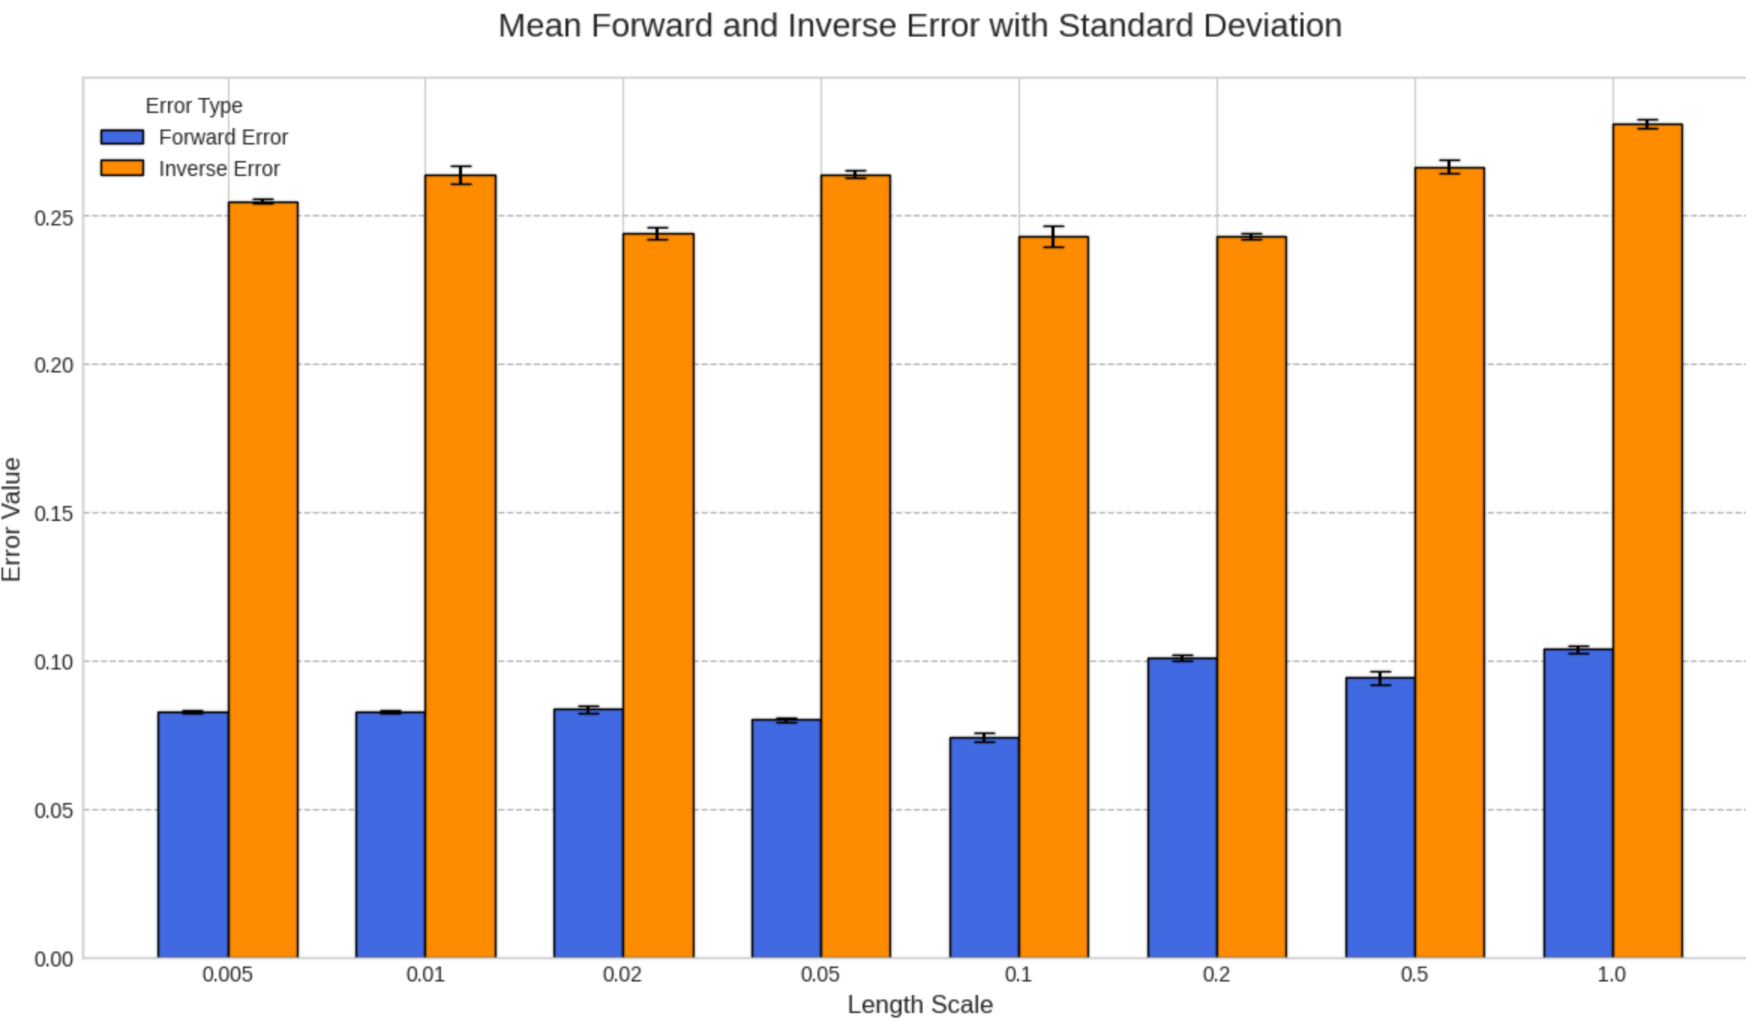
\includegraphics[height=15em]{len_darcy_1d.png}
\caption{Relative \(L^{2}\)-error of forward and inverse tasks for the 1D Darcy flow problem as the length scale  varies for the Gaussian process noise. Means and standard deviations are plotted across three inference runs.}\label{fig:d1dlen}
\end{figure}

From this, we see that the ``sweet spot'' hypothesis in \Cref{sec:design1} is confirmed: there is an ideal length scale

% \subsection{Noise smoothness}
% We first experiment with

% Narrative for 1D goes as follows:
% \begin{enumerate}
%   \item to choose roughness of noise, look at graph of relative L2 error when projecting 1D dataset onto the RKHS of \(C\) for RBF kernel of different length scales
%   \item compare this to empirical results when training on differnet length scales
%   \item show experiment with time re-weightings and argue that the time change \(\theta(t) = t^{2}\) is best -- it outperforms even the ease-in-out schedule which we attribute to \textit{starvation} of the intermediate time steps
%   \item having establisehd \(\theta(t) = t^{2}\) as the best time change, show experiment where \(t\) is sampled according to \(u^{2}\) where \(u \sim \operatorname{U}[0, 1]\). This does not perform as well which we attribute to \textit{model starvation} -- not enough emphasis on crucial earlier time steps. hence we argue that the change-in-time is there primarily to mitigate the explosion in the coefficient on \(\eta\) and thus preventing amplification of training errors
%   \item compare with the "alternative parameterisation" where we only learn \(\mathop{\mathbb{E}}\qty[\xi_{1} \mid \xi_{0}, x_{t}]\) and show this does not work well
%   \item hence for the expensive 2D datasets we go ahead with uniform time sampling during training, and learn \(\varphi, \eta\)
% \end{enumerate}
\section{2D Dataset}\label{sec:darcy2}

% Narrative for 2D datasets goes as follows
% \begin{enumerate}
%   \item present results for different length scales
%   \item compare performance with FunDPS and vanilla stochatic interpolants baselines and show performance is very competitive with the former and (hopefully) far exceeds that of the latter
%   \item ablation: training the marginal model. performance not much worse, so it's useful in circumstances where we want to train less and are willing to give up some performance. likely due to diffusion paths being mainly driven by the conditioning on \(x_{t}\) not \(\xi_{0}\)
%   \item ablation: ODE. note that we can predict \(\xi_{1}\) given \(\xi_{0}\) using only one step. haven't yet done this experiment
% \end{enumerate}

% TODOs: dynamic sensors, sparse sensors
% TODOs: higher res inference for 2D
%\include{Chapter5/chapter5}
%\include{Chapter6/chapter6}
%\include{Chapter7/chapter7}

% ********************************** Back Matter *******************************
% Backmatter should be commented out, if you are using appendices after References
%\backmatter

% ********************************** Bibliography ******************************
\begin{spacing}{0.9}

  % To use the conventional natbib style referencing
  % Bibliography style previews: http://nodonn.tipido.net/bibstyle.php
  % Reference styles: http://sites.stat.psu.edu/~surajit/present/bib.htm

  \bibliographystyle{apalike}
  %\bibliographystyle{unsrt} % Use for unsorted references
  %\bibliographystyle{plainnat} % use this to have URLs listed in References
  \cleardoublepage
  \bibliography{References/references} % Path to your References.bib file

  % If you would like to use BibLaTeX for your references, pass `custombib' as
  % an option in the document class. The location of 'reference.bib' should be
  % specified in the preamble.tex file in the custombib section.
  % Comment out the lines related to natbib above and uncomment the following line.

  %\printbibliography[heading=bibintoc, title={References}]

\end{spacing}

% ********************************** Appendices ********************************

\begin{appendices} % Using appendices environment for more functunality

  %!TEX root = ../thesis.tex
% ******************************* Thesis Appendix A ****************************
\chapter{Mathematical Proofs} \label{app:A}

\section{Proof of \Cref{lem:fpmarg}}\label{prf:lem:fpmarg}
\restatelemfpmarg*

\begin{proof}
  It is sufficient to restrict our attention to any real-valued test function of the form \(u(t, x) = \operatorname{Re}\qty[\phi(t) e^{i \ev{x, h(t)}_{H}}]\) or \(\operatorname{Im}\qty[\phi(t) e^{i \ev{x, h(t)}_{H}}]\), where \(\phi\) and \(h\) satisfy the properties given in \Cref{eqn:testfns}.

  Fix \(t \in [0,1]\) and consider the characteristic function of the real-valued random variable \(u(t, x_{t})\). For any \(k \in \mathbb{R}\), we define
  \begin{align}
    \chi(t, k) &\coloneqq \mathop{\mathbb{E}}\qty[e^{i k u(t, x_{t})}]
  \end{align}
  Taking derivatives with respect to \(t\) and \(k\) and evaluating at \(k=0\) allows us to compute the time derivative of the expected value of \(u(t, x_{t})\):
  \begin{equation}
    %   \pdv{t}\chi(t, k) &= i k \mathop{\mathbb{E}}\qty[e^{i k u(t, x_{t})} \qty(D_{t} u(t, x_{t}) + \ev{ \dot{x}_{t}, D_{x}u(t, x_{t})}_{H})] \\
    \eval{\frac{1}{i} \pdv[2]{}{t}{k} \chi(t, k)}_{k=0} = \dv{t} \mathop{\mathbb{E}}\qty[u(t, x_{t})] = \mathop{\mathbb{E}}\qty[D_{t} u(t, x_{t}) + \ev{ \dot{x}_{t}, D_{x}u(t, x_{t})}_{H}].
  \end{equation}

  Since the inner product \(\ev{ \dot{x}_{t}, D_{x} u(t, x_{t})}_{H}\) is linear in its first argument, we may apply the law of iterated expectations and replace \(\dot{x}_{t}\) with \(\zeta(t, x_{t}) = \mathop{\mathbb{E}}\qty[ \dot{x}_{t} \mid x_{t}]\) as defined in \Cref{eqn:zetadef}:
  \[
    \dv{t} \mathop{\mathbb{E}}\qty[u(t, x_{t})] = \mathop{\mathbb{E}}\qty[D_{t} u(t, x_{t}) + \ev{  \zeta(t, x_{t}), D_{x} u(t, x_{t})}_{H}]
  \]

  Adding and subtracting \(\frac{\varepsilon}{\gamma(t)} \eta(t, x_{t})\), where \(\eta(t, x_{t}) = \mathop{\mathbb{E}}\qty[ z \mid x_{t}]\) as defined in \Cref{eqn:etadef}, we have
  \begin{align}
    \dv{t} \mathop{\mathbb{E}}\qty[u(t, x_{t})] &= \mathop{\mathbb{E}}\qty[D_{t} u(t, x_{t}) + \ev{ \frac{\varepsilon}{\gamma(t)}\eta(t, x_{t}) + \zeta(t, x_{t}) - \frac{\varepsilon}{\gamma(t)} \eta(t, x_{t}), D_{x} u(t, x_{t})}_{H}] \notag \\
    &= \frac{\varepsilon}{\gamma(t)}\mathop{\mathbb{E}}\qty[\ev{z, D_{x}u(t, x_{t})}_{H}] + \mathop{\mathbb{E}}\qty[ D_{t}u(t, x_{t}) + \ev{f(t, x_{t}), D_{x} u(t, x_{t})}_{H}], \label{eqn:simpl}
  \end{align}
  where we simplified the first term using the law of iterated expectations to simplify the first term, and substituted the definition \(f(t, x) = \zeta(t, x) - \frac{\varepsilon}{\gamma(t)} \eta(t, x)\) given in \Cref{eqn:deff} for the second term.

  For the following, we assume that \(u(t, x) = \operatorname{Re}[\phi(t) e^{i \ev{x, h(t)}_{H}}]\), but an identical line of reasoning applies if \(u(t, x) = \operatorname{Im}\qty[\phi(t) e^{i \ev{x, h(t)}_{H}}]\).

  Let us focus on the first term in \Cref{eqn:simpl}. We have:
  \begin{align}
    \frac{\varepsilon}{\gamma(t)} \mathop{\mathbb{E}}[\ev{z, D_{x} u(t, x_{t})}_{H}] &= \operatorname{Re}\qty[i \frac{\varepsilon}{\gamma(t)} \mathop{\mathbb{E}}\qty[\phi(t) e^{i \ev{x_{t}, h(t)}_{H}} \ev{z, h(t)}_{H}]] \notag \\
    &= \operatorname{Re}\qty[i \frac{\varepsilon}{\gamma^{2}(t)} \mathop{\mathbb{E}}\qty[\phi(t) e^{i \ev{\alpha(t) \xi_{0} + \beta(t) \xi_{1}, h(t)}_{H}}] \mathop{\mathbb{E}}\qty[e^{i \ev{\gamma(t) z, h(t)}_{H}} \ev{\gamma(t) z, h(t)}_{H}]], \label{eqn:nearlythere}
  \end{align}
  where the second line follows since \(z \perp (\xi_{0}, \xi_{1})\).

  Let \(\qty{\lambda_{n}, e_{n}}_{n=1}^{\infty}\) be an orthonormal system for \(C\) (i.e. \(C e_{n} = \lambda e_{n}\) for each \(n\)) and define the scalar-valued functions \(h_{n}(t) \coloneqq \ev{h(t), e_{n}}_{H}\). The projections \(z_{n} = \ev{z, e_{n}}\) for each \(n\) are mutually independent 1-dimensional Gaussians with zero mean and variances equal to \(\lambda_{n}\).  By Parseval's theorem, we have the identity \(\ev{\gamma(t) z, h(t)} = \sum_{n=1}^{\infty} \gamma(t) h_{n}(t) z_{n} \). We may therefore write
  \[
    \mathop{\mathbb{E}}\qty[\ev{\gamma(t) z, h(t)}_{H} e^{i \ev{\gamma(t)z, h(t)}_{H}}] = \sum_{n=1}^{\infty} \mathop{\mathbb{E}}\qty[\gamma(t) h_{n}(t) z_{n} e^{i \gamma(t) h_{n}(t) z_{n}}] \prod\limits_{m \neq n} \mathop{\mathbb{E}}\qty[e^{i \gamma(t) h_{m}(t) z_{m}}]
  \]
  Using the identity \(\mathop{\mathbb{E}}\qty[q e^{i q}] = i v \mathop{\mathbb{E}}\qty[e^{i q}]\) for a 1-dimensional Gaussian \(v \sim \operatorname{N}(0, q)\), we have
  \begin{align*}
    \mathop{\mathbb{E}}\qty[\ev{\gamma(t) z, h(t)}_{H} e^{i \ev{\gamma(t)z, h(t)}_{H}}] = \sum_{n=1}^{\infty} i \gamma^{2}(t)h_{n}^{2}(t)\lambda_{n} \mathop{\mathbb{E}}\qty[e^{i \ev{\gamma(t) z, h(t)}_{H}}]
  \end{align*}
  Substituting into \Cref{eqn:nearlythere}, we have
  \begin{align*}
    \frac{\varepsilon}{\gamma(t)} \mathop{\mathbb{E}}\qty[\ev{z, D_{x} u(t, x_{t})}_{H}] &= \mathop{\mathbb{E}}\qty[\sum_{n=1}^{\infty} - \varepsilon \lambda_{n} h_{n}^{2}(t) u(t, x_{t})] = \mathop{\mathbb{E}}\qty[\operatorname{Tr}\qty(\varepsilon C D^{2}_{x}u(t, x_{t}))].
  \end{align*}
  Finally, substituting this expression into \Cref{eqn:simpl} and re-writing expectations via integrals, we have
  \[
    \dv{t} \int_{H} u(t, x) \mu_{t}(\dd{x}) = \int_{H} \operatorname{Tr}\qty(\varepsilon C D^{2}_{x} u(t, x)) + D_{t}u(t, x) + \ev{f(t, x), D_{x}u(t, x)}_{H} \mu_{t}(\dd{x}).
  \]
  Since the choice of \(t\) was arbitrary, it follows that \(\mu_{t}\) satisfies the Fokker-Plank equation (\ref{eqn:fp}) for any \(t \in [0, t]\). This concludes the proof.
\end{proof}

\section{Proof of \Cref{thm:mbsde}}\label{prf:thm:mbsde}
\restatethmmbsde*
\begin{proof}
  In addition to \(\nu\), we define the measures \(\rho\) and \(\mu\) on the product space \([0, \overline{t}] \times H\) determined uniquely by \(\rho(\dd{(t, x)}) = \rho_{t}(\dd{x}) \dd{t}\) and \(\mu(\dd{(t, x)}) = \mu_{t}(\dd{x}) \dd{t}\). Hence, it follows by construction that \(\nu = \frac{1}{2} \rho + \frac{1}{2} \nu\) and both \(\rho\)and \(\mu\) are absolutely continuous with respect to \(\nu\). We define their densities \(p, q\) with respect to \(\nu\):
  \[
    p(t, x) \coloneqq \dv{\rho}{\nu}(t, x) \qand q(t, x) = \dv{\mu}{\nu}(t, x).
  \]
  From \Cref{lem:fpmarg} we know that both \(\rho_{t}\) and \(\mu_{t}\) solve the Fokker-Plank equation (\ref{eqn:fp}). Hence,
  \begin{equation}
    0 = \int_{[0, \overline{t}] \times H} \mathcal{L} u(t, x) (p(t, x)  -q(t, x)) \nu(\dd{(t, x)}) \label{eqn:fpuniq}
  \end{equation}
  for every test function \(u \in E\). Note that for \(\nu\)-almost every \((t, x)\), we have \(0 \leq p(t, x), q(t, x) \leq 2\), so their difference is bounded almost everywhere. Since \Cref{eqn:fpuniq} holds for every \(u \in E\) and by assumption, \(\mathcal{L} E\) is dense in \(L^{1}([0, \overline{t}] \times H, \nu)\), it follows that
  \[
    p(t, x) = q(t, x)
  \]
  for \(\nu\)-almost every \((t, x)\). Hence, the signed measure \(\rho - \mu = 0\) and \(\rho_{t} = \mu_{t}\) for \(\dd{t}\)-almost every \(t\). This  concludes the proof.
\end{proof}
% TODO: remove eqn numbers where they are redundant

% TODO: ensure all ev's have a _H or H_c, etc

\section{Proof of \Cref{lem:bayes}}\label{prf:lem:bayes}
\restatelembayes*

% TODO: must summarise steps in the proof
\begin{proof}
  The proof proceeds in steps TODO
  \paragraph{Step 0}
  Let \(\mu_{1 \mid 0, t}(\dd{\xi_{1}}, x_{0}, x)\) denote the posterior law of \(\xi_{1}\), conditional on \(\xi_{0} = x_{0}\) and \(x_{t} = x\). Furthermore, let \(\mathbb{P}_{1 \mid 0}(\dd{\xi_{1}}, x_{0})\) be the corresponding conditional prior, which is a well-defined Gaussian measure on \(H_{C}\)  (see, e.g., \citealp[][Chapter 3.10]{bogachev1998gaussian}). We use \(m_{1 \mid 0}(x_{0})\) and \(Q_{1 \mid 0}\) respectively to denote the mean and covariance operator of this Gaussian on \(H_{C}\). Note that the prior conditional mean \(m_{1 \mid 0}(x_{0})\) is a linear function of \(x_{0}\). Then for \(\mu_{0}\)-almost every \(x_{0} \in H_{C}\), the law \(\mu_{1 \mid 0, t}(\dd{\xi_{1}, x_{0}, x})\) is absolutely continuous with respect to the reference measure \(\mathbb{P}_{1 \mid 0}(\dd{\xi_{1}}, x_{0})\) with the following density:
  \begin{align*}
    \dv{\mu_{1 \mid 0, t}(\cdot, x_{0}, x)}{\mathbb{P}_{1 \mid 0}(\cdot, x_{0})}{}(\xi_{1}) &= \frac{1}{Z_{1 \mid 0,t}(x_{0}, x)}\exp(- V_{1 \mid 0, t}(\xi_{1}, x_{0}, x)),\\
    \text{ where } V_{1 \mid 0, t}(\xi_{1}, x_{0}, x) &\coloneqq \frac{1}{2\gamma^{2}(t)} \norm{\alpha(t) x_{0}+ \beta(t) \xi_{1} - x}_{H_{C}}^{2} + \Phi(x_{0}, \xi_{1}),
  \end{align*}
  and \(Z_{1 \mid 0,t}(x_{0}, x) \coloneqq \int_{H_{C}} \exp(- V_{1 \mid 0, t}(\xi_{1}, x_{0}, x)) \mathbb{P}_{1 \mid 0} (\dd{\xi_{1}, x_{0}})\) is a normalising constant.
  \paragraph{Step 1} Let \(\qty{e_{n}}_{n=1}^{\infty}\) be an orthonormal basis for \(H_{C}\) and for each \(N \geq 1\), let \(H_{N}\) be the linear span of \(\qty{e_{1}, \ldots, e_{N}}\). We define \(\Pi_{N} : H_{C} \to H_{N}\) as the self-adjoint orthogonal projection operator onto the finite-dimensional subspace \(H_{N}\) of \(H_{C}\) and let \(\xi_{1,N} \coloneqq \Pi_{N} \xi_{1}\). Furthermore, we define a reference measure by projecting \(\mathbb{P}_{1 \mid 0}\) onto this subspace:
  \begin{align*}
    \mathbb{P}_{1 \mid 0, N}(\dd{\xi_{1, N}}, x_{0}) &\coloneqq \operatorname{N}(m_{1 \mid 0, N}(x_{0}),  Q_{N}), \\
    \text{ where } m_{1 \mid 0, N}(x_{0}) &\coloneqq \Pi_{N} m_{1 \mid 0}(x_{0}), \\
    \text{ and } Q_{N} &\coloneqq \Pi_{N} Q_{1 \mid 0} \Pi _{N}.
  \end{align*}
  Using this, we create a sequence of approximating posterior measures \(\mu_{1 \mid 0, t, N}\) by restricting the potential to \(H_{N}\): for each \(\xi_{1,N} \in H_{N}\).
  \begin{align*}
    \dv{\mu_{1 \mid 0, t, N}(\cdot, x_{0}, x)}{\mathbb{P}_{1 \mid 0, N}(\cdot, x_{0})}{}(\xi_{1,N}) &\coloneqq \frac{1}{Z_{1 \mid 0, t, N}(x_{0}, x)} \exp(-V_{1 \mid 0, t, N}(\xi_{1,N}, x_{0}, x)), \\
    \text{ where } V_{1 \mid 0, t, N}(\xi_{1, N}, x_{0}, x) &\coloneqq  \frac{1}{2\gamma^{2}(t)} \norm{\alpha(t) \Pi_{N} x_{0} + \beta(t) \xi_{1, N} - x}^{2}_{H_{C}} + \Phi(x_{0}, \xi_{1, N}),
  \end{align*}
  where \(Z_{1 \mid 0, t, N}(x_{0}, x) \coloneqq \int_{H_{N}} \exp(-V_{1 \mid 0, t, N})(\xi_{1, N}, x_{0}, x) \mathbb{P}_{1 \mid 0, N}(\dd{\xi_{1, N}, x_{0}})\) is a normalising constant.

  Given these definitions, we study the following approximation of the posterior mean:
  \begin{equation}
    m_{1 \mid 0, t, N}(x_{0}, x) \coloneqq \mathop{\mathbb{E}_{\mu_{1 \mid 0, t, N}(\cdot, x_{0}, x)}}\qty[\xi_{1, N}] = \int_{H_{N}} \xi_{1, N}\mu_{1 \mid 0, t, N}(\dd{\xi_{1, N}}, x_{0}, x).\label{eqn:apm}
  \end{equation}
  We aim to find a Lipschitz constant for the map \(x \mapsto m_{1 \mid 0, t, N}(x_{0}, x)\) that is independent of \(N\) and \(x_{0}\). To do so, we consider the Frechet derivative of \(m_{1 \mid 0, t, N}(x_{0}, x)\) with respect to \(x\), applied in a direction \(h \in H_{C}\). This is a covariance (see Lemma \ref{lem:frechetf}):

  \begin{align}
    D_{x} m_{1 \mid 0, t, N}(x_{0}, x)[h] &=\frac{\beta(t)}{\gamma^{2}(t)} \mathop{\mathbb{E}_{\mu_{1 \mid 0, t, N}(\cdot, x_{0}, x)}}\qty[(\xi_{1, N} - m_{1 \mid 0, t, N}(x_{0}, x)) \ev{\xi_{1, N} - m_{1 \mid 0, t, N}(x_{0}, x), h}_{H_{C}}] \notag \\
    &=\frac{\beta(t)}{\gamma^{2}(t)} \mathop{\mathbb{E}_{\mu_{1 \mid 0, t, N}(\cdot, x_{0}, x)}}\qty[(\xi_{1, N} - m_{1 \mid 0, t, N}(x_{0}, x)) \ev{\xi_{1, N} - m_{1 \mid 0, t, N}(x_{0}, x), \Pi_{N} h}_{H_{N}}] \label{eqn:dxmt0},
  \end{align}
  where the second equality follows from the first since the components of \(\xi_{1, N} - m_{1 \mid 0, t, N}(x_{0}, x)\) along the basis vectors \(\qty{e_{n}}_{n=N+1}^{\infty}\) are all zero.

  By the Riesz representation theorem, the \(N\)-dimensional subspace \(H_{N}\) is isomorphic with \(\mathbb{R}^{N}\), so all vectors on \(H_{N}\) can be identified with an \(N\)-dimensional column vector in \(\mathbb{R}^{N}\). We may therefore re-write the derivative using an \(N\)-dimensional covariance matrix \(C_{N}\) acting on the vector \(\Pi_{N} h\):
  \begin{align}
    D_{x} m_{1 \mid 0, t, N}(x_{0}, x)[h] &= \frac{\beta(t)}{\gamma^{2}(t)} C_{N} \Pi_{N} h, \label{eqn:dxmt}\\
    \text{ where } C_{N} &= \mathop{\mathbb{E}_{\mu_{1 \mid 0, t, N}(\cdot, x_{0}, x)}}\qty((\xi_{1, N} - m_{1 \mid 0, t, N}(x_{0}, x))(\xi_{1, N} - m_{1 \mid 0, t, N}(x_{0}, x))^{\tran}). \notag
  \end{align}
  For the rest of the proof, we identify \(C_{N}\) with a self-adjoint covariance operator on \(H_{N}\).

  \paragraph{Step 2}
  We now use the Brascamp-Lieb inequality \citep{brascamp1976extensions} to place a bound on the operator norm of \(C_{N}\). We proceed by expressing the approximate posterior measure \(\mathbb{\mu}_{1 \mid 0, t, N}(\dd{\xi_{1, N}}, x_{0}, x)\) via a density relative to the Lebesgue measure on \(H_{N}\) (identified with \(\mathbb{R}^{N}\)). The density of the reference measure \(\mathbb{P}_{1 \mid 0, N}(\dd{\xi_{1, N}}, x_{0})\) with respect to the Lebesgue measure, evaluated at \(\xi_{1, N} \in H_{N}\), is proportional to
  \[\exp(-\frac{1}{2} \ev{Q_{N}^{-1} (\xi_{1, N} - m_{1 \mid 0, N}(x_{0})), \xi_{1, N} - m_{1 \mid 0, N}(x_{0})}_{H_{N}}),
  \]
  where the inverse \(Q_{N}^{-1}\) is well-defined because \(Q_{N} : H_{N} \to H_{N}\) is positive-definite and bounded. Hence, % TODO: refer back to the theorem
  \begin{align*}
    &\mu_{1 \mid 0, t, N}(\dd{\xi_{1, N}}, x_{0}, x) \\
    &\quad\propto \exp(-V_{1 \mid 0, t, N}(\xi_{1, N}, x_{0}, x) - \frac{1}{2} \ev{Q_{N}^{-1} (\xi_{1, N} - m_{1 \mid 0, N}(x_{0})), \xi_{1, N} - m_{1 \mid 0, N}(x_{0})}_{H_{N}}) \dd{\xi_{1, N}}.
  \end{align*}
  Let \(W_{1 \mid 0, t, N}(\xi_{1, N}, x_{0}, x) \coloneqq V_{1 \mid 0, t, N}(\xi_{1, N}, x_{0}, x) + \frac{1}{2} \ev{Q_{N}^{-1} (\xi_{1, N} - m_{1 \mid 0, N}(x_{0})), \xi_{1, N} - m_{1 \mid 0, N}(x_{0})}_{H_{N}}\)  be the total potential with respect to the Lebesgue measure on \(H_{N}\). Since this is twice-differentiable and strictly convex, the conditions for the Brascamp-Lieb inequality are satisfied (see \citep[][Theorem 4.1]{brascamp1976extensions}): for any continuously differentiable function \(f : H_{N} \to \mathbb{R}\), we have
  \begin{align*}
    &\mathop{\mathbb{E}_{\mu_{1 \mid 0, t, N}(\cdot, x_{0}, x)}}\qty[\qty(f(\xi_{1, N}) - \bar{f})^{2}]\\
    &\quad\leq \mathop{\mathbb{E}_{\mu_{1 \mid 0, t, N}(\cdot, x_{0}, x)}}\qty[\ev{ \qty(D^{2}_{\xi_{1, N}}W_{1 \mid 0, t, N}(\xi_{1, N}, x_{0}, x))^{-1} D f(\xi_{1, N}), D f(\xi_{1, N}) }_{H_{N}}],
  \end{align*}
  where \(\overline{f}\) is the expectation of \(f(\xi_{1, N})\) under the measure \(\mu_{1 \mid 0, t, N}(\dd{\xi_{1, N}, x_{0}, x})\) and \(D^{2}_{\xi_{1, N}}W_{1 \mid 0, t, N}(\xi_{1, N}, x_{0}, x)\) is the inverse Hessian of \(W_{1 \mid 0, t, N}(\xi_{1, N}, x_{0}, x)\) with respect to \(\xi_{1, N}\) on \(H_{N}\). In the case where \(f(\xi_{1, N}) = \ev{\xi_{1, N}, u}_{H_{N}}\) for any \(u \in H_{N}\), we have \(Df(\xi_{1, N}) = u\), and
  \begin{align}
    &\mathop{\mathbb{E}_{\mu_{1 \mid 0, t, N}(\cdot, x_{0}, x)}}\qty[\qty(f(\xi_{1, N}) - \bar{f})^{2}] = \ev{C_{N}u, u} \notag\\
    &\qquad\qquad\leq  \mathop{\mathbb{E}_{\mu_{1 \mid 0, t, N}(\cdot, x_{0}, x)}}\qty[\ev{ \qty(D^{2}_{\xi_{1, N}}W_{1 \mid 0, t, N}(\xi_{1, N}, x_{0}, x))^{-1} u, u }_{H_{N}}]. \label{eqn:brascamp}
  \end{align}
  \paragraph{Step 3}
  We now aim to place a Loewner order on the inverse Hessian \(\qty(D^{2}_{\xi_{1, N}}W_{1 \mid 0, t, N}(\xi_{1, N}, x_{0}, x))^{-1}\) irrespective of \(\xi_{1, N}\), which will in turn allow us to form a Loewner order on \(C_{N}\).

  Taking the second-order Frechet derivatives of \(W_{1 \mid 0, t,N}(\xi_{1, N}, x_{0}, x)\) with respect to \(\xi_{1, N}\) in the directions \(u, v \in H_{N}\), we have
  \begin{align*}
    D^{2}_{\xi_{1, N}}W_{1 \mid 0, t, N}(\xi_{N}, x_{0}, x)[u, v] = \ev{\qty(\frac{\beta^{2}(t)}{\gamma^{2}(t)} I_{N} + \Pi_{N}\grad_{\xi_{1}}^{2}\Phi(x_{0}, \xi_{1, N})\Pi_{N} + Q_{N}^{-1})u, v}_{H_{N}},
  \end{align*}
  where \(\grad_{\xi_{1}}^{2} \Phi(\xi_{0}, \xi_{1})\) is the partial Hessian of the potential \(\Phi\) with respect to the second coordinate. This allows us to identify the Hessian with a self-adjoint Hessian operator from \(H_{N}\) to \(H_{N}\):
  \begin{equation}
    D^{2}_{\xi_{1, N}}W_{1 \mid 0, t, N}(\xi_{N}, x_{0}, x)[u, v] = \frac{\beta^{2}(t)}{\gamma^{2}(t)} I_{N} + \Pi_{N}\grad_{\xi_{1}}^{2}\Phi(x_{0}, \xi_{1, N})\Pi_{N} + Q_{N}^{-1}\label{eqn:hess}
  \end{equation}
  Since \(\Phi\) is \(k\)-strongly convex, it is also \(k\)-strongly convex in the second coordinate and hence the projection of its partial Hessian satisfies the following Loewner order:
  \[
    \Pi_{N} \grad^{2}_{\xi_{1}} \Phi(x_{0}, \xi_{1, N}) \succcurlyeq k I_{N},
  \]
  which allows us to place a Loewner order on \Cref{eqn:hess}:
  \[
    D^{2}_{\xi_{1, N}}W_{1 \mid 0, t, N}(\xi_{N}, x_{0}, x)[u, v] \succcurlyeq \qty(\frac{\beta^{2}(t)}{\gamma^{2}(t)} + k) I_{N} + Q_{N}^{-1}
  \]
  Since the right-hand side of this quantity is positive-definite, this Loewner order is reversed when taking inverses:
  \[
    \qty(D^{2}_{\xi_{1, N}}W_{1 \mid 0, t, N}(\xi_{N}, x_{0}, x)[u, v])^{-1} \preccurlyeq \qty(\qty(\frac{\beta^{2}(t)}{\gamma^{2}(t)} + k) I_{N} + Q_{N}^{-1})^{-1}.
  \]
  This relationship holds uniformly for all \(\xi_{1, N} \in H_{N}\). Substituting into \Cref{eqn:brascamp}, we have
  \begin{align*}
    \ev{C_{N}u, u} &\leq \ev{\qty(\qty(\frac{\beta^{2}(t)}{\gamma^{2}(t)} + k) I_{N} + Q_{N}^{-1})^{-1}u, u}_{H_{N}}, \text{ for all } u \in H_{N}\\
    \iff C_{N} &\preccurlyeq \qty(\qty(\frac{\beta^{2}(t)}{\gamma^{2}(t)} + k) I_{N} + Q_{N}^{-1})^{-1}.
  \end{align*}
  \paragraph{Step 4} Having established a Loewner order on \(C_{N}\), we now use this to place a bound on the operator norm of \(C_{N}\). Since \(C_{N}\) is positive semi-definite, the Loewner order translates directly into an ordering on operator norms:
  \[
    \onorm{C_{N}} \leq \onorm{\qty(\qty(\frac{\beta^{2}(t)}{\gamma^{2}(t)} + k) I_{N} + Q_{N}^{-1})^{-1}}.
  \] % TODO: add operator norm to nomenclature
  The spectrum of the operator \(\qty(\qty(\frac{\beta^{2}(t)}{\gamma^{2}(t)} + k) I_{N} + Q_{N}^{-1})^{-1}\) is given by the function \(\sigma(\lambda) = \frac{\lambda \gamma^{2}(t)}{\lambda (\beta^{2}(t) + k \gamma^{2}(t)) + \gamma^{2}(t)}\) evaluated over the spectrum of \(Q_{N}\). This function is monotone and increasing for \(\lambda \geq 0\), attaining its supremum at \(\frac{\gamma^{2}(t)}{\beta^{2}(t) + k \gamma^{2}(t)}\). Hence, we have
  \[
    \onorm{C_{N}} \leq \frac{\gamma^{2}(t)}{\beta^{2}(t) + k \gamma^{2}(t)} \leq \frac{\gamma^{2}(t)}{\beta^{2}(t)}.
  \] Substituting this relationship in \Cref{eqn:dxmt},
  \begin{align*}
    \norm{D_{x} m_{1 \mid 0, t, N}(x_{0}, x)[h]}_{H_{C}} &\leq \frac{\beta(t)}{\gamma^{2}(t)} \onorm{C_{N}} \onorm{\Pi_{N}} \norm{h}_{H_{C}} \leq \frac{1}{\beta(t)} \norm{h}_{H_{C}}.
  \end{align*}
  It follows from the mean-value inequality \citep[][Theorem 2.1.19]{berger1977nonlinearity}, that for any \(x, y \in H\),
  \begin{equation}
    \norm{m_{1 \mid 0, t, N}(x_{0}, x) - m_{1 \mid 0, t, N}(x_{0}, y)}_{H_{C}} = \norm{m_{1 \mid 0, t, N}(x_{0}, x) - m_{1 \mid 0, t, N}(x_{0}, y)}_{H_{N}} \leq \frac{1}{\beta(t)} \norm{x - y}_{H_{C}}. \label{eqn:ineq}
  \end{equation}%
  Passing \(N \to \infty\), the sequence of approximate posterior means \(m_{1 \mid 0, t, N}(x_{0}, x)\) converges to the true posterior mean \(m_{1 \mid 0, N}(x_{0}, x)\) (see Lemma \ref{lem:posteriormeanconvergence}). Since each approximation satisfies the inequality (\ref{eqn:ineq}) that is uniform in \(N\) and the norm is a continuous mapping, the true posterior mean \(m_{1 \mid 0, t}(x_{0}, x)\) also inherits inequality.
  \[
    \norm{m_{1 \mid 0, t}(x_{0}, x) - m_{1 \mid 0, t}(x_{0}, y)}_{H_{C}} \leq \frac{1}{\beta(t)} \norm{x - y}_{H_{C}}.
  \]
  This concludes the proof.%

  %
  % TODO: add and cite brascamp-Lieb
  % TODO: explain why approximate posteriormeans converge
  %
  %Finally, note that at \(t = 0\), the posterior mean \(m_{1 \mid 0, t}(x_{0}, x)\) collapses to \(\mathop{\mathbb{E}}\qty[\xi_{1} \mid \xi_{0} = x_{0}]\) when \(x = x_{0}\) and is undefined when \(x \neq x_{0}\). We extend its definition at time \(t=0\) to equal \(\mathop{\mathbb{E}}\qty[\xi_{1} \mid \xi_{0}]\) even when \(x_{0} \neq x\). With this extension, the Lipscchitz continuity holds also in the case where \(t = 0\) since it no longer changes with \(x\).
  %
  % TODO: Frechet derivative in nomenclature
  %
\end{proof}

\begin{lemma}\label{lem:frechetf}
  Let \(m_{1 \mid 0, t, N}(x_{0}, x)\) be an approximate posterior mean as defined in \Cref{eqn:apm}, with \(t \in(0,1)\) and \(N \geq 0\). Then the Frechet derivative of the mapping \(x \mapsto m_{1 \| 0, t, N}(x_{0}, x)\) in \(H_{C}\)-norm, in a direction \(h \in H_{C}\) is given by
  \[
    D_{x} m_{1 \mid 0, t, N}(x_{0}, x)[h] =\frac{\beta(t)}{\gamma^{2}(t)} \mathop{\mathbb{E}_{\mu_{1 \mid 0, t, N}(\cdot, x_{0}, x)}}\qty[(\xi_{1, N} - m_{1 \mid 0, t, N}(x_{0}, x)) \ev{\xi_{1, N} - m_{1 \mid 0, t, N}(x_{0}, x), h}_{H_{C}}]
  \]

  \begin{proof}
    We begin by taking the Frechet derivative of \(m_{1 \mid 0, t, N}(x_{0}, x)\) at \(x\) in a direction \(h \in H_{C}\). Applying the quotient rule (see \citealp[][Chapter 2.1]{berger1977nonlinearity}) and simplifying, we have
    \begin{align}
      D_{x} m_{1 \mid 0, t, N}(x_{0}, x)[h] &= D_{x}\qty{\frac{\int_{H_{N}} \xi_{1, N} \exp(-V_{1 \mid 0, t, N}(\xi_{1, N},x_{0}, x)) \mathbb{P}_{1 \mid 0, N}(\dd{\xi_{1, N}}, x_{0})}{ Z_{1 \mid 0, t, N}(x_{0}, x)}}[h] \notag \\
      &= \frac{1}{Z_{1 \mid 0, t, N}(x_{0}, x)} D_{x}U_{1 \mid 0, t, N}(x_{0}, x)[h] - m_{1 \mid 0, t, N}(x_{0}, x) \frac{D_{x} Z_{1 \mid 0, t, N}(x_{0}, x)[h]}{Z_{1 \mid 0, t, N}(x_{0}, x)}, \label{eqn:lem10fin}
    \end{align}
    where we define \(U_{1 \mid 0, t, N}(x _{0}, x) \coloneqq \int_{H_{N}} \xi_{1, N} \exp(-V_{1 \mid 0, t, N}(\xi_{1, N},x_{0}, x)) \mathbb{P}_{1 \mid 0, N}(\dd{\xi_{1, N}}, x_{0})\) to simplify notation. Evaluating the Frechet derivatives, we have
    \begin{align*}
      D_{x}U_{1 \mid 0, t, N}(x_{0}, x)[h] &= \frac{1}{\gamma^{2}(t)}\int_{H_{N}} \xi_{1, N} \ev{\alpha(t) \Pi_{N} x_{0} + \beta(t) \xi_{1, N} - x, h}_{H_{C}}\\[-0.5em]
      &\qquad \qquad \cdot \exp(-V_{1 \mid 0, t, N}(\xi_{1, N}, x_{0}, x)) \mathbb{P}_{1 \mid 0, N}(\dd{\xi_{1, N}}, x_{0}), \\
      D_{x} Z_{1 \mid 0, t, N}(x_{0}, x)[h] &= \frac{1}{\gamma^{2}(t)}\int_{H_{N}} \ev{\alpha(t) \Pi_{N} x_{0} + \beta(t) \xi_{1, N} - x, h}_{H_{C}} \\[-0.5em]
      &\qquad \qquad \cdot \exp(-V_{1 \mid 0, t, N}(\xi_{1, N}, x_{0}, x)) \mathbb{P}_{1 \mid 0, N}(\dd{\xi_{1, N}}, x_{0}).
    \end{align*}
    Substituting these into \Cref{eqn:lem10fin} and recognising that the fractions come together to form the approximate posterior density, we have:
    \[
      D_{x} m_{1 \mid 0, t, N}(x_{0}, x)[h] = \frac{1}{\gamma^{2}(t)}\mathop{\mathbb{E}_{\mu_{1 \mid 0, t, N}(\cdot, x_{0}, x)}}\qty[(\xi_{1, N} - m_{1 \mid 0, t, N}(x_{0}, x))\ev{\alpha(t) \Pi_{N} x_{0} + \beta(t) \xi_{1, N} - x, h}_{H_{C}}].
    \]
    Adding and subtracting zero,
    \[
      0 = \frac{1}{\gamma^{2}(t)} \mathop{\mathbb{E}_{\mu_{1 \mid 0, t ,N}(\cdot, x_{0}, x)}}\qty[(\xi_{1, N} - m_{1 \mid 0, t, N}(x_{0}, x)) \ev{- \alpha(t) \Pi_{N} x_{0}  + \beta(t) m_{1 \mid 0, t, N}(x_{0}, x) + x, h}_{H_{C}}],
    \]
    we arrive at the expression
    \[
      D_{x} m_{1 \mid 0, t, N}(x_{0}, x)[h] = \frac{\beta(t)}{\gamma^{2}(t)}\mathop{\mathbb{E}_{\mu_{1 \mid 0, t, N}(\cdot, x_{0}, x)}}\qty[(\xi_{1, N} - m_{1 \mid 0, t, N}(x_{0}, x))\ev{\xi_{1, N} - m_{1 \mid 0, t, N}(x_{0}, x), h}_{H_{C}}].
    \]
    This concludes the proof.
  \end{proof}
\end{lemma}

\begin{lemma}\label{lem:posteriormeanconvergence}
  Let \(\qty{m_{1 \mid 0, t, N}(x_{0}, x)}_{N=1}^{\infty}\)  be a sequence of approximate posterior means as defined in \Cref{eqn:apm}, with \(t \in (0, 1)\). Then for almost every \(x_{0}, x\), the sequence converges to the true posterior mean \(m_{1 \mid 0, t}(x_{0}, x)\).

  \begin{proof}
    First, let us re-express the definition of \(m_{1 \mid 0, t, N}(x_{0}, x)\) by lifting the integrals into a common infinite-dimensional space:
    \begin{align}
      m_{1 \mid 0, t, N}( x_{0}, x) &= \int_{H_{C}} \Pi_{N} \xi_{1} \frac{1}{Z_{1 \mid 0, t, N}(x_{0}, x)} \exp(-V_{1 \mid 0, t}(\Pi_{N} \xi_{1}, \Pi_{N} x_{0}, x)) \mathbb{P}_{1 \mid 0}(\dd{\xi_{1}}, x_{0}),  \label{eqn:lift}\\
      \text{ where } Z_{1 \mid 0, t, N}(x_{0}, x) &= \int_{H_{C}} V_{1 \mid 0, t}(\Pi_{N} \xi_{1}, \Pi_{N} x_{0}, x) \mathbb{P}_{1 \mid 0}(\dd{\xi_{1}}, x_{0}).\notag
    \end{align}

    We define the sequence of functions \[f_{N}(\xi_{1}) \coloneqq \Pi_{N} \xi_{1} \frac{1}{Z_{1 \mid 0, t, N}(x_{0}, x)}\exp(- V_{1 \mid 0, t}(\Pi_{N} \xi_{1}, \Pi_{N} x_{0}, x)),\] and \[f(\xi_{1}) \coloneqq \xi \frac{1}{Z_{1 \mid 0, t}(x_{0}, x)}\exp(-V_{1 \mid 0, t}(\xi_{1}, x_{0}, x)),\] for fixed \(x_{0}\) and  \(x\). To show convergence, we appeal to the Vitali convergence theorem \citep{walnut2011vitali}, which is a generalisation of the dominated convergence theorem and states that if the sequence of functions \(f_{N}\) is pointwise-convergent to \(f\) and uniformly integrable, then the integral of the functions also converges to the integral of \(f\). We proceed in two steps: we first show pointwise convergence, and then show uniform integrability.

    \paragraph{Step 1: Pointwise Convergence} The numerator \(\Pi_{N} \xi_{1} \exp(-V_{1 \mid 0, t}(\Pi_{N} \xi_{1}, \Pi_{N} x_{0}, x))\) is clearly pointwise convergent to \(\xi_{1} \exp(-V_{1 \mid 0, t}(\xi_{1}, x_{0}, x))\) since for any fixed \(\xi_{1} \in H_{C}\), the projection \(\Pi_{N} \xi_{1}\) converges to \(\xi_{1}\) in \(H_{C}\)-norm, and \(V_{1 \mid 0, t, x}\) is continuous in all of its inputs. Hence, it remains to show convergence of the sequence of normalising constants \(Z_{1 \mid 0, t, N}(x_{0}, x)\).

    To this end, we apply the dominated convergence theorem to show that
    \[
      \lim\limits_{N \to \infty} \int_{H_{C}} \exp(-V_{1 \mid 0}(\Pi_{N} \xi_{1}, \Pi_{N} x_{0}, x)) \mathbb{P}_{1 \mid 0}(x_{0}) = \lim\limits_{N \to \infty} \int_{H_{C}} \exp(-V_{1 \mid 0}(\xi_{1}, x_{0}, x)) \mathbb{P}_{1 \mid 0}(\dd{\xi_{1}}, x_{0}).
    \]
    Since \(\Phi\) is strongly convex, it has a unique global minimum. This implies that the integrand on both sides are bounded by a constant \(M_{1} < \infty\) that does not depend on \(N\). Since the constant function is integrable on any probability space, it follows from the dominated convergence theorem that \(\lim\limits_{N \to \infty} Z_{1 \mid 0, t, N}(x_{0}, x) = Z_{1 \mid 0, t}(x_{0}, x)\).

    Finally, since the normalising constant is nonzero for any \(N\) and converges to a non-zero value, the functions \(f_{N}(\xi_{1})\) are pointwise convergent to \(f(\xi_{1})\).

    \paragraph{Step 2: Uniform Integrability}
    A sufficient condition for uniform integrability is that there exists a uniform bound on the expected squared norm of sequence of the functions \(f_{N}\) \citep[][Theorem 3.5]{billingsley2013convergence}:
    \begin{equation}
      \int_{H_{C}} \norm{\Pi_{N} \xi_{1}}_{H_{C}}^{2} \frac{1}{Z_{1 \mid 0, t, N}^{2}(x_{0}, x)} \exp(-2 V_{1 \mid 0, t}(\Pi_{N} \xi_{1}, \Pi_{N} x_{0}, x)) \mathbb{P}_{1 \mid0}(\dd{\xi_{1}}, x_{0}). \label{eqn:dc2}
    \end{equation}
    We will again employ the dominated convergence theorem to show that this sequence converges, and hence is bounded. First, pointwise convergence holds trivially since both the numerator and denominators converge, and the squared normalising factors \(Z^{2}_{1 \mid 0, t, N}(x_{0}, x)\) are positive for all \(N\) and converge to a positive value. Furthermore, the integrand is uniformly bounded by a constant \(\overline{M}\), since the strong convexity of \(\Phi\) ensures that the potential grows at least quadratically as \(\norm{\Pi_{N} \xi_{1}}_{H_{C}} \to \infty\) and hence overwhelms the quadratic growth of the \(\norm{\Pi_{N} \xi_{1}}^{2}_{H_{C}}\) pre-factor.

    The dominated convergence theroem therefore applies and it follows that the sequence of integrals in \Cref{eqn:dc2} is convergent and therefore bounded. Hence, the sequence of functions \(f_{N}\) is uniformly integrable.

    Since we have shown that the sequence of functions \(f_{N}\) is pointwise convergent and uniformly integrable, it follows that their integrals, which are equal to the approximate posterior means \(m_{1 \mid 0, t, N}(x_{0}, x)\), are convergent and converge to the true posterior mean \(m_{1 \mid 0, t}(x_{0}, x)\).
  \end{proof}
\end{lemma}

% \begin{lemma}\label{lem:aposteriormeancont}
%   Let \(\qty{m_{1 \mid 0, t, N}(x_{0}, x)}_{N=1}^{\infty}\)  be a sequence of approximate posterior means as defined in \Cref{eqn:apm}, with \(t \in (0, 1)\). For every \(N \geq 1\), the mapping \(x \mapsto m_{1 \mid 0, t, N}(x_{0}, x)\) is continuous in \(H_{C}\)-norm.

%   \begin{proof}
%     Let \(\qty{x_{j}}_{j=1}^{\infty}\) be a convergent sequence, converging to a vector \(x\) in \(H_{C}\)-norm. We apply the dominated convergence theorem to show that the corresponding sequence of approximate posterior means \(\qty{m_{1 \mid 0, t, N}(x_{0}, x_{j})}_{j=1}^{\infty}\) also converge in \(H_{C}\)-norm. Since the dominating arguments are identical to those in \Cref{lem:posteriormeanconvergence}, we provide only a sketch of a proof here.

%     We first lift the defining integrals for the approximate posterior means \(m_{1 \mid 0, t, N}(x_{0}, x)\) to integrals over a common infinite-dimensional space as in \Cref{lem:posteriormeanconvergence} (see Equation \ref{eqn:lift}). Since the potential \(V_{1 \mid 0, t}(\Pi_{N}, \xi_{1}, \Pi_{N}, x_{0}, x)\) is continuous in \(x\), an application of the dominated convergence theorem shows that the normaling constants converge as \(j \to \infty\). Hence, the integrands for the approximate posterior means converge pointwise. Again, the strong-convexity of \(\Phi\) implies a uniform bound on this integrand. A second application of the dominated convergence theorem hence implies convergence of the approximate posterior means: \(\lim\limits_{j \to \infty} m_{1 \mid 0, t, N}(x_{0}, x_{j}) = m_{1 \mid 0, t, N}(x_{0}, x)\). This concludes the proof.
%   \end{proof}
% \end{lemma}

% Since the arguments in the proof to \Cref{lem:aposteriormeancont} do not depend on the dimension of the orthogonal projection \(N\), they apply also to the true posterior mean. Hence, the true posterior mean is also continuous in the conditioning variable \(x_{t} =x\). We state this below as a corollary.

% \begin{corollary}
%   The true posterior mean \(m_{1 \mid 0, t}(x_{0}, x) = \mathop{\mathbb{E}}\qty[\xi_{1} \mid \xi_{0} = x_{0}, x_{t} = x]\) is continuous in \(x\), in \(H_{C}\)-norm.
% \end{corollary}

\section{Proof of \Cref{lem:manifold}}
Our proof follows a similar overarching argument to to proof of \Cref{lem:bayes} in \Cref{prf:lem:bayes}: we find a bound for the expression for the Frechet derivative of the posterior mean, expressed as a covariance. The assumption of bounded support in \(H_{C}\) norm allows us to greatly simplify our arguments which we apply directly in infinite dimensions.

As in \Cref{prf:lem:bayes}, we let \(\mu_{1 \mid 0, t}(\dd{\xi_{1}}, x_{0}, x)\) denote the posterior law of \(\xi_{1}\), conditional on \(\xi_{0} = x_{0}\) and \(x_{t} = x\). This time however, for each \(t \in (0, 1)\) we let the reference measure be \(\mathbb{P}_{t} \coloneqq \operatorname{N}(0, \gamma^{2}(t) C)\). Note that the Cameron-Martin space of \(\gamma^{2}(t)C\) is identical to of \(C\), equipped with an inner product scaled by \(\frac{1}{\gamma^{2}(t)}\). Since \(\alpha(t)\xi_{0} + \beta(t) \xi_{1}\) is supported in \(H_{C}\) and hence also the Cameron-Martin space of \(\gamma^{2}(t)(C)\) \(H_{\gamma^{2}(t)C}\), the measure \(\mu_{1 \mid 0, t}(\dd{\xi_{1}}, x_{0}, x)\) is absolutely continuous with respect to \(\mathbb{P}_{t}\):
\begin{align*}
  \dv{\mu_{1 \mid 0, t}(\cdot, x_{0}, x)}{\mathbb{P}_{t}}{}(\xi_{1}) &= \frac{1}{Z_{1 \mid 0, t}(x_{0}, x)}\exp(-V_{1 \mid 0, t}(\xi_{1}, x_{0}, x)), \\
  \text{ where } V_{1 \mid 0, t}(\xi_{1}, x_{0}, x) &= \frac{1}{\gamma^{2}} \norm{\alpha(t) x_{0} + \beta(t) \xi_{1} - x}_{H_{C}}^{2},
\end{align*}
and \(Z_{1 \mid 0, t}(x_{0}, x) \coloneqq \int_{H_{C}} \exp(-V_{1 \mid 0, t}(\xi_{1}, x_{0}, x)) \mathbb{P}_{t}(\dd{\xi_{1}})\) is a normalising constant. Defining \(m_{t}(x_{0}, x)\) as the posterior mean:
\[
  m_{t}(x_{0}, x) \coloneqq \mathop{\mathbb{E}_{\mu_{1 \mid 0, t}(\cdot, x_{0}, x)}}\qty[\xi_{1}] = \int_{H_{C}} \xi_{1} \mu_{1 \mid 0, t}(\dd{\xi_{1}}, x_{0}, x),
\]
we take the Frechet derivative in the direction \(h \in H_{C}\), we again arrive at a covariance:
\[
  D_{x} m_{t}(x_{0}, x)[h] = \frac{\beta(t)}{\gamma^{2}(t)} \mathop{\mathbb{E}_{\mu_{1 \mid 0, t}(\cdot, x_{0}, x)}}\qty[ (\xi_{1} - m_{t}(x_{0}, x))\ev{\xi_{1} - m_{t}(x_{0}, x), h}_{H_{C}} \mu_{1 \mid 0, t}]
\]
Taking the norm in \(H_{C}\) and applying the Cauchy-Schwarz inequality, we have
\[
  \norm{D_{x} m_{t}(x_{0}, x)[h]}_{H_{C}} \leq \frac{\beta(t)}{\gamma^{2}(t)} \mathop{\mathbb{E}_{\mu_{1 \mid 0, t}(\cdot, x_{0}, x)}}\qty[\norm{\xi_{1} - m_{t}(x_{0}, x)}_{H_{C}}^{2}] \norm{h}_{H_{C}}
\]
Using the fact that \(0 \leq \mathop{\mathbb{E}}\qty[\norm{\xi_{1} - m_{t}(x_{0}, x)}_{H_{C}}^{2}] = \mathop{\mathbb{E}}\qty[\norm{\xi_{1}}_{H_{C}}^{2}] - \norm{m_{t}(x_{0}, x)}^{2}\) and \(\norm{\xi_{1}^{2}}_{H_{C}} \leq R^{2}\) almost surely, we conclude
\[
  \norm{D_{x} m_{t}(x_{0}, x)[h]}_{H_{C}} \leq \frac{R^{2} \beta(t)}{\gamma^{2}(t)} \norm{h}_{H_{C}}.
\]
Finally, since the coefficient on \(\norm{h}_{H_{C}}\) is uniform in \(h\), we apply the mean-value inequality and conclude that \(m_{t}(x_{0}, x)\) is Lipschitz in \(H_{C}\)-norm with Lipschitz inequality at most \(\frac{R^{2}\beta(t)}{\gamma^{2}(t)}\):
\[
  \norm{m_{t}(x_{0}, x) - m_{t}(x_{0}, y)}_{H_{C}} \leq \frac{R^{2}\beta(t)}{\gamma^{2}(t)} \norm{x - y}_{H_{C}}.
\]
This concludes the proof.
  %!TEX root = ../thesis.tex
% ******************************* Thesis Appendix B ********************************

\chapter{Network Architecture}\label{app:B}
\section{1D Darcy Problem}
Below, we detail the hyperparameters we used when training our FNO networks for the 1D Darcy flow problem (Section \ref{sec:prelim}).

\end{appendices}

% *************************************** Index ********************************
\printthesisindex % If index is present

\end{document}
